% -*- coding:utf-8 mod:LaTeX -*-
% !TeX spellcheck = de_DE
%Neue deutsche Trennmuster
%Siehe http://www.ctan.org/pkg/dehyph-exptl und http://projekte.dante.de/Trennmuster/WebHome
%Nur für pdflatex, nicht für lualatex
% \RequirePackage[ngerman=ngerman-x-latest]{hyphsubst}
%Warns about outdated packages and missing caption declarations
%See https://www.ctan.org/pkg/nag
\RequirePackage[l2tabu, orthodox]{nag}
% TODO: b5?
% \documentclass[paper=a5,twoside,fontsize=10pt, DIV=calc, headings=small, bibliography=totoc, listof=totoc]{scrbook}
\documentclass[paper=a4,twoside,fontsize=10pt, DIV=calc, headings=small, bibliography=totoc, listof=totoc]{scrbook}
\usepackage[utf8]{inputenc}

\usepackage[acronym,indexonlyfirst,nomain]{glossaries}
\makeglossaries
%%% languages
\newacronym{openmp}{OpenMP}{Open Multi-Processing}
\newacronym{hpx}{HPX}{High Performance ParalleX}
\newacronym{cuda}{CUDA}{Compute Unified Device Architecture}
\newacronym{hip}{HIP}{Heterogeneous-computing Interface for Portability}
\newacronym{opencl}{OpenCL}{Open Computing Language}

\newacronym{hpc}{HPC}{High Performance Computing}
\newacronym{vm}{VM}{Virtual Machine}
\newacronym{simd}{SIMD}{Single Instruction Multiple Data}
\newacronym{mpi}{MPI}{Message Passing Interface}
\newacronym{ci}{CI}{Continuous Integration}

\input{shared/template}
\usepackage{shared/titlepage}

\usepackage{geometry}
\geometry{
    paper=b5paper,
    inner=16mm,         % Inner margin
    outer=24mm,         % Outer margin
    bindingoffset=10mm, % Binding offset
    top=20mm,           % Top margin
    bottom=28mm,        % Bottom margin
    %showframe,         % show how the type block is set on the page
}

\usepackage[newfloat]{minted}
% Add the following lines, wherever you want.
\makeatletter
\AddToHook{begindocument/before}{\@ifpackageloaded{minted}{\removefromtoclist[float]{lol}}{}}
\makeatother
\setminted{
    breaklines,%
    linenos,%
    escapeinside=@@,%
    highlightcolor=GreenYellow,%
}

\usepackage{siunitx}
\sisetup{
  per-mode=fraction,
  fraction-function=\tfrac
}
\DeclareSIUnit{\flop}{FLOP}
\DeclareSIUnit{\flops}{FLOPS}
\DeclareSIUnit{\transfer}{T}

\usepackage{tikz}
\usetikzlibrary{external, decorations.pathreplacing}
\tikzexternalize[prefix=tikz/]

%use TODO with \todo{}
\setlength {\marginparwidth }{2cm}
\usepackage{todonotes}
\LetLtxMacro{\oldtodo}{\todo}
\renewcommand{\todo}[2][]{\tikzexternaldisable\oldtodo[inline, #1]{#2}\tikzexternalenable}



\usepackage[amsmath, hyperref]{ntheorem}
\usepackage{csquotes}
\usepackage{mathrsfs}
\usepackage{phoenician}
\usepackage{interval}
\usepackage{makecell}
\usepackage{booktabs}
\usepackage{tabularray}
\UseTblrLibrary{booktabs}
\usepackage{fontawesome5}
\usepackage[most]{tcolorbox}
\usepackage{threeparttable}
\usepackage{pgf}
\usepackage{pgfplots}

\DeclarePairedDelimiter\abs{\lvert}{\rvert}%
\DeclarePairedDelimiter\norm{\lVert}{\rVert}%

% % Command to use in Math Mode
% \newcommand{\pp}{\reflectbox{$\mathrm{P}$}\mkern-7mu\mathrm{P}}
% % Command to use in text
% \newcommand{\ppm}{$\pp$\xspace}

% % Command to use in Math Mode
% \newcommand{\mpp}{\overline{\reflectbox{$\mathrm{P}$}\mkern-7mu\mathrm{P}}}
% % Command to use in text
% \newcommand{\mppm}{$\mpp$\xspace}

% Performance Portability Metric
\newcommand{\pp}{\ensuremath{\reflectbox{$\mathrm{P}$}\mkern-7mu\mathrm{P}}\xspace}
% Marowka Performance Portability Metric
\newcommand{\mpp}{\ensuremath{\overline{\reflectbox{$\mathrm{P}$}\mkern-7mu\mathrm{P}}}\xspace}

\newmintinline[code]{cpp}{}

\newcommand{\cpp}[1][]{C\nolinebreak\hspace{-.05em}\raisebox{.4ex}{\tiny\bfseries +}\nolinebreak\hspace{-.10em}\raisebox{.4ex}{\tiny\bfseries +}#1\xspace}
\newcommand{\dpcpp}{DPC\nolinebreak\hspace{-.05em}\raisebox{.4ex}{\tiny\bfseries +}\nolinebreak\hspace{-.10em}\raisebox{.4ex}{\tiny\bfseries +}\xspace}
\newcommand{\charmpp}{Charm\nolinebreak\hspace{-.05em}\raisebox{.4ex}{\tiny\bfseries +}\nolinebreak\hspace{-.10em}\raisebox{.4ex}{\tiny\bfseries +}\xspace}
\newcommand{\qdppp}{QDP\nolinebreak\hspace{-.05em}\raisebox{.4ex}{\tiny\bfseries +}\nolinebreak\hspace{-.10em}\raisebox{.4ex}{\tiny\bfseries +}\xspace}

\newcommand{\setfontsize}[1]{\fontsize{#1pt}{1.2\dimexpr#1pt\relax}\selectfont}

\newcolumntype{C}[1]{>{\centering\arraybackslash}p{#1}}

% Define a custom box for advantages
\newtcolorbox{advantagebox}[1]{
    colback=green!10!white,
    colframe=green!50!black,
    title=\textbf{Advantages},
    fonttitle=\bfseries,
    rounded corners,
    boxrule=0.8pt,
    equal height group=#1
}

% Define a custom box for disadvantages
\newtcolorbox{disadvantagebox}[1]{
    colback=red!10!white,
    colframe=red!50!black,
    title=\textbf{Disadvantages},
    fonttitle=\bfseries,
    rounded corners,
    boxrule=0.8pt,
    equal height group=#1
}

% Combine an advantage and a disadvantage box
\newcommand{\AdvantagesAndDisadvantages}[3]{
\noindent
\begin{minipage}[t]{0.49\textwidth}
    \vspace{0pt}
    \begin{advantagebox}{#1}
        \begin{itemize}[leftmargin=2.5mm]
            \setlength\itemsep{0.0em}
            #2
        \end{itemize}
    \end{advantagebox}
\end{minipage}
\hfill
\begin{minipage}[t]{0.49\textwidth}
    \vspace{0pt}
    \begin{disadvantagebox}{#1}
        \begin{itemize}[leftmargin=2.5mm]
            \setlength\itemsep{0.0em}
            #3
        \end{itemize}
    \end{disadvantagebox}
\end{minipage}\newline
}

% nicely typeset quotes
\NewDocumentEnvironment{quotebox}{m b}
{%
    \vspace{0.2\baselineskip} % Top margin
    \begin{quote}\itshape
      \enquote{#2} % Main content (third argument)
      \newline\raggedleft --- #1 % Mandatory author (first argument)
    \end{quote}
    \vspace{0.2\baselineskip} % Bottom margin
}%
{%
}%

% Define a modern-looking code block style
\tcbuselibrary{minted}  % Unicode support for minted
\newtcblisting{moderncode}[2][]{
    listing engine=minted,
    colframe=black!50,    % Subtle border
    coltitle=black,       % Title color
    boxrule=0.5pt,        % Thin border
    arc=3pt,              % Slightly rounded corners
    boxsep=5pt,           % Padding for readability
    listing only,         % Ensures only code is displayed
    minted language=#2,   % Default language (can be overridden)
    minted options={xleftmargin=8pt, #1},
}


% binding correction
\setlength{\evensidemargin}{-24pt}
\setlength{\oddsidemargin}{-24pt}
\renewcommand{\lstlistingname}{Code}
\renewcommand{\listingname}{Code}
\renewcommand{\listingautorefname}{Listing}
\newcommand{\autoquotename}{Quote}
\newcommand{\definitionautorefname}{Definition}





\includeonly{content/02_performance_portability}

%\input{commands}

\bibliography{bibliography}

% \hyphenation{
% Spe-zi-fi-ka-tion
% In-te-gra-tion
% An-for-de-rung An-for-de-run-gen
% Be-nut-zer-ober-flä-che
% Mes-sung-en
% aus-zu-tau-schen
% Lauf-zeit-in-for-ma-tionen
% % Dürfen nicht getrennt werden
% AROMA TOSCA BPMN OASIS OMG DMTF IT DevOps
% }

\begin{document}
\iftex4ht
\Configure{graphics*}  % After begin document. Package tex4ht
  {pdf}
  {\Link[\csname Gin@base\endcsname .png]{}{}% link the png
  \Picture[pict]{\csname Gin@base\endcsname .png width:80\% align=center border=0}%  Show the png
  \EndLink
  }

\Css{body {text-align:justify;}}

%all LaTeX formulas as pictures
\Configure{$}{\PicMath}{\EndPicMath}{}
%$ % <- syntax highlighting fix for emacs
\fi

%Tipp von http://goemonx.blogspot.de/2012/01/pdflatex-ligaturen-und-copynpaste.html
%siehe auch http://tex.stackexchange.com/questions/4397/make-ligatures-in-linux-libertine-copyable-and-searchable
%
%ONLY WORKS ON MiKTeX
%On other systems, download glyphtounicode.tex from http://pdftex.sarovar.org/misc/
%
\input glyphtounicode.tex
\pdfgentounicode=1

% Die Seitennummerierung erfolgt durchlaufend ab der Titelseite. Also keine
% Spielereien mit römischen Ziffern usw. - Die ISO 7144 schreibt das sogar für
% wissenschaftliche Werke vor.
% Von Promitionsordnung verlangt!
% Deshalb ist \frontmatter DEAKTIVIERT
%\frontmatter
\title{Thesis Title}
%\author{\texorpdfstring{\href{http://www.example.org/}{Author Name}}{Author Name}}
\author{Marcel Breyer}
\date{\today}
\keywords{TODO}
\firstexaminer{Prof.~Dr.~Dirk Pflüger}
\secondexaminer{Prof.~Dr.~???}
\dateofexamination{unbekannt}
\placeofbirth{Waiblingen}
\faculty{Fakultät für Informatik, Elektrotechnik und Informationstechnik}
\department{Institut für Parallel und Verteilte Systeme}

\maketitle

% This is necessary if you have more than 9 sections/subsections/subsubsections
% \makeatletter
% \renewcommand\l@section{\@dottedtocline{1}{1.5em}{3em}}
% \renewcommand\l@subsection{\@dottedtocline{2}{1.5em}{4.3em}}
% \renewcommand\l@subsubsection{\@dottedtocline{3}{1.5em}{5.6em}}
% \makeatother

\tableofcontents
\clearpage

\pagestyle{justpagenums}
% \input{abstract}

%\mainmatter
\pagestyle{scrheadings}

%% --- Zusammenfassung ---------------------------------------------
\include{content/_01_Zusammenfassung}

%% --- Abstract Page---------------------------------------------
\include{content/_02_abstract}

%% --- Acknowledgements page------------------------------------
\include{content/_03_acknowledgements}

\pagestyle{scrheadings}

%% --- CONTENT ---

% TODO: which hardware used where

\include{content/01_introduction}
\chapter{Performance Portability}

\todo{3-P challenge: performance, portability, and productivity}

\section{What Is Performance?}
\label{sec:performance}

Understanding the meaning of \textit{performance} is key to assessing performance portability. 
When looking at the Cambridge Dictionary entry of the word performance, we can see a few different definitions based on the context\footnote{\url{https://dictionary.cambridge.org/dictionary/english/performance} (visited: 2025-03-31)}:
\begin{description}
    \item[activity:] \enquote{how well a person, machine, etc. does a piece of work or an activity}
    \item[entertainment:] \enquote{the action of entertaining other people by dancing, singing, acting, or playing music}
    \item[doing:] \enquote{the act of doing something, such as your job}
    \item[business:] \enquote{how successful an investment, company, etc. is and how much profit it makes}
\end{description}
From these short examples, we can already see that \enquote{a good performance} heavily depends on the context. 
This is also true for performance in the computer science domain. 
For example, when asking machine learners about the performance of their \gls{ml} models, they will answer with different model metrics showing how well their model performs on new, unseen data. 
On the other hand, if you ask a member of the \gls{hpc} community about the performance of their, e.g., simulation, we will most likely get an answer regarding the total walltime the simulation needed to complete or the achieved memory bandwidth. 
\citet{pennycook_implications_2019} defined \textit{performance} in their work as   
\begin{quotebox}{\citet{pennycook_implications_2019}}
    Any measurable property of an application’s correct execution of a problem on a platform.
\end{quotebox}
This definition is so broad that it can be used for both of the above computer science domain examples. 
In the remainder of this dissertation, I will stick to the context of \gls{hpc} when discussing performance. 

However, even in this context, there is no single widely agreed-upon definition or metric for describing the performance of some code. 
Possible metrics can include, but are not limited to:
\begin{description}
    \item[walltime:] Also known as \textbf{runtime} or \textbf{time-to-solution}, the time a code needs to finish its execution.
    \item[throughput:] The rate of finished processing tasks (depending on the problem at hand), an example could be the number of lattice updates.
    \item[scalability:] The, e.g., strong or weak scaling behavior of an application when increasing the number of available compute resources.
    \item[utilization:] The degree to which the available compute resources are used. 
    \item[efficiency:] The efficiency of the code which can include walltime, but also other metrics like the amount of used memory or the energy consumption. 
\end{description}
When we look at this list, we can see that the transitions between the categories are fluent. 
For example, a high efficiency most likely also correlates with a high compute utilization and a small walltime, while a high memory throughput also correlates with high memory utilization. 
Additionally, most metrics need some baseline to compare against, like hardware-specific limits or another application we want our application. 

However, most of the time, one or more of three basic metrics are used: walltime, \glspl{flops}, and attained memory bandwidth. 
Collecting walltimes is straightforward and can directly be done in the used programming language using built-in features like \cpp's date and time \code{<chrono>} library. 
However, gathering the achieved \glspl{flops} or memory bandwidth is more difficult. 
Additionally, the theoretical peak performance must also be known to calculate the reached compute or memory efficiency. 
While this is generally easier for \glspl{gpu} since most vendors publish these performance values, it is more difficult for \glspl{cpu} since these values are generally not provided. 
Therefore, in the following two sections, I will introduce how to estimate the theoretical and achieved \gls{flops} and memory bandwidth for a given compute node and application. 
Both will be needed later to calculate the performance efficiency of the investigated applications. 

\subsection{Estimating the Floating Point Operations per Second}
\label{sec:perf:peak_flops}

\citet{dolbeau_theoretical_2018} provides a tutorial on how to calculate the theoretical peak performance in \gls{flops} of modern \glspl{cpu} factoring in modern \gls{cpu} features like hyper-threading, clock boosts, vectorization, or \gls{fma} units. 
He splits the calculation into two basic categories: the \gls{cpu}'s micro-architecture, fixed for a core of a given micro-architecture, and the machine-architecture, which depends on the actual \gls{cpu} model and compute node setup. 

The first micro-architecture characteristic is the \textit{floating point operations per compute operation} where mostly the cheap floating point operations like addition, subtraction, and multiplication are counted as $\frac{1}{1}$. 
Modern \glspl{cpu} also include \gls{fma} units that are capable of calculating $d = a \cdot b + c$ in a single instruction, which is counted as $\frac{2}{1}$.
Next are the \textit{compute operations per instructions}, which depend on the available vectorization standards and floating point type (FP32 vs. FP64). 
For example, for scalar only execution, the count would be $\frac{1}{1}$ independent of the floating point type; for \gls{avx} 512, it would be $\frac{16}{1}$ for single precision FP32 and $\frac{8}{1}$ for double precision FP64. 
Last are the \textit{instructions per cycle} accounting for potential superscalar execution. 
If a \gls{cpu} supports two scalar or \gls{fma} operations simultaneously, the count would for example be $\frac{2}{1}$, if a scalar operation can be simultaneously executed with a \gls{fma} operation, the count can be encompassed as $\frac{3}{2}$.

The machine-architecture characteristics seem to be easier to gather at first, but this may not necessarily hold for modern \glspl{cpu}. 
The \textit{cycles per second} corresponds to the \gls{cpu}'s frequency. 
However, care must be taken since modern \glspl{cpu} have different frequencies depending on turbo modes, power saving options, thermal throttling, and whether \gls{avx} instructions are used. 
Since \gls{avx} is always assumed to be used in the theoretical considerations, the most sensible value would be the \gls{avx} all-core frequency. 
Next are the \textit{cores per socket}, where only physical cores should be used since hyper-threading does not add new resources. 
Last are the \textit{sockets per node} in modern multi-socket systems. 

Putting all these characteristics together into one formula results in the \autoref{def:peak_flops} provided by~\citet{dolbeau_theoretical_2018}.
\begin{definition}[\gls{flops} per Node~\cite{dolbeau_theoretical_2018}]\label{def:peak_flops}
Given the micro-architecture and machine-architecture characteristics of a \gls{cpu}, the theoretical peak \acrfull{flops} for a compute node can be calculated using
$$ \frac{flops}{node} = \frac{flop}{operation} \cdot \frac{operations}{instruction} \cdot \frac{instructions}{cycle} \cdot \frac{cycles}{second} \cdot \frac{cores}{socket} \cdot \frac{sockets}{node} $$
\begin{tikzpicture}
    \node at (0, 0) {}; % dummy node that placement works correctly
    \draw[transform canvas={yshift=1.1cm}, decorate,decoration={brace, amplitude=8pt, mirror, raise=6ex}] (1.85, 0) -- (8, 0) node[midway, yshift=-4.5em]{\text{micro-architecture}};
    \draw[transform canvas={yshift=1.1cm}, decorate,decoration={brace, amplitude=8pt, mirror, raise=6ex}] (8, 0) -- (11.9, 0) node[midway, yshift=-4.5em]{\text{machine-architecture}};
\end{tikzpicture}
\vspace{-1cm}
\end{definition}
Note that this calculated theoretical peak \gls{flops} only serves as a sensible upper bound. 
A real-world example will not be guaranteed or even likely to achieve the calculated theoretical peak performance. 
Nevertheless, if all researchers agree on one way to calculate the theoretical peak \gls{flops}, it can be used as a baseline, making results between different papers more easily comparable. 

As an example, we compute the theoretical peak \gls{flops} for double precision floating point types and a machine with dual-socket \gls{amd} EPYC 9274F \glspl{cpu}~\cite{amd_amd_2022}, which will also be used as a hardware platform in the later chapters. 
This \gls{cpu} has support for \gls{fma}3 and \gls{avx}-512. 
However, in Zen4 \gls{avx}-512 is implemented by \enquote{double-pumping} two $\SI{256}{\bit}$ registers. 
This means that the \gls{avx}-512 unit can compute one \gls{fma} instruction in two consecutive clock cycles, resulting in a count of $\frac{2}{2}$~\cite{amd_amd_2023}. 
Additionally, the EPYC 9274F \glspl{cpu} has an all-core frequency of $\SI{4.1}{\giga\hertz}$ and $\num{24}$ physical cores. 
Therefore, according to \autoref{def:peak_flops}, the theoretical peak \gls{flops} of the example machine's dual-socket \gls{cpu} are: $2 \cdot 8 \cdot 1 \cdot \SI{4.1}{\giga\hertz} \cdot 24 \cdot 2 = \SI{3148.8}{\giga\flops}$.

To get a more empirical upper bound and to verify if our theoretical peak \gls{flops} do indeed make sense, we can use one of the standard \gls{hpc} benchmarks like the \gls{hpl} benchmark~\cite{petitet_hpl_2018}. 
In the case of the EPYC 9274F \gls{cpu}, I used the \gls{amd} provided pre-built \gls{hpl} version~\cite{amd_pre-built_2025} and ran it with the default settings. 
As a result, the utility reported a performance of $\SI{2765.6}{\giga\flops}$, which is only $\SI{12}{\percent}$ worse than our theoretically calculated value. 
This shows us that our theoretical peak \gls{flops} are not too conservative and do not dramatically overestimate the possible real-world performance of our \gls{cpu}. 

If we are interested in the actually achieved performance in \gls{flops}, we have two options. 
First, we can use a tool that automatically provides us with the \gls{flops} values when we execute our code, like NVIDIA's nvprof~\cite{nvidia_corporation_cuda_2025}, \gls{amd}'s rocprofv3~\cite{amd_using_2024}, or likwid-perfctr~\cite{thomas_gruber_likwid_2023}. 
Alternatively, if no such tool is available or the current programming framework or hardware platform is not supported, we can calculate the necessary floating point operations by hand and divide it by the elapsed walltime. 
However, we must be careful when doing so. 
For example, if our target hardware supports \gls{fma} operations, we have to count code that looks like, e.g., \code{c[i] += a[i] * b[i]} as a single floating point operation. 
Additionally, counting the number of floating point instructions for non-trivial operations like floating point divisions, square roots, or exponential functions is difficult. 
Such operations can be translated into a single machine instruction with higher-than-normal latency or throughput, a fixed number of machine instructions, or even a variable number of machine instructions. 
In practice, these operations are often counted as a single instruction. 
To get a better estimate, we would have to examine the generated assembly code to count the number of floating-point instructions that are actually generated. 

\begin{listing}
    \begin{moderncode}{cpp}
#pragma omp parallel for
for (std::size_t i = 0; i < N; ++i) {
    a[i] = b[i] + q * c[i];
}
    \end{moderncode}
    \caption{%
    The standard vector TRIAD function from the STREAM benchmark suite~\cite{mccalpin_memory_1995}. 
    }
    \label{code:stream_triad}
\end{listing}

For example, let's look at the TRIAD function from the STREAM benchmark suite~\cite{mccalpin_memory_1995} shown in \autoref{code:stream_triad}. 
We can see two floating point operations, a multiplication and an addition; however, since our example \gls{amd} EPYC 9274F \gls{cpu} supports \gls{fma} operations, we have to count these operations as a single instruction. 
Therefore, the number of floating point operations in \autoref{code:stream_triad} is directly based on the number of loop iterations \code{N}. 
Running this code with \code{N=1e12} on our dual-socket \gls{amd} EPYC 9274F \gls{cpu} machine results in a runtime of $\SI{1.308}{\second}$, which means $\SI{11.47}{\giga\flop}$. 
The same code profiled with likwid-perfctr reports $\SI{0}{\giga\flop}$. 


\todo{Beispiel stream/triad CPU benchmark + likwid output $\rightarrow$ verifizieren, dass die Berechnung halbwegs sinnvoll ist!}

\todo{sinnvolles beispiel}
\subsection{Estimating the Memory Bandwidth}
\label{sec:perf:mem_bandwidth}


If we are interested in the actually achieved memory bandwidth, we can use the same method as for the achieved \gls{flops}.
The previously presented utilities can also be used to gather the attained memory bandwidth. 
Alternatively, we can count the number of transferred bytes. 
Again, we must be careful what to count since not all variable access results in a memory transfer. 

Looking at the TRIAD function again \autoref{code:stream_triad}, we have to load three FP64 values per iteration, resulting in $\SI{24}{\byte}$ loaded per iteration and $\SI{240}{\giga\byte}$ in total. 
Since the execution took $\SI{1.308}{\second}$, we have an achieved memory bandwidth of $\SI{183.49}{\giga\byte\per\second}$. 
\section{The Hardware Sampling Library: hws}

\cite{breyer_hws_2024}
\cite{breyer_hardware-independent_2024} % poster

\begin{itemize}
    \item \cpp with Python bindings using Pybind11 \cite{jakob_pybind11_2017}
    % \item CPUs via trubostat, lscpu, free \cite{brown_turbostat_nodate, qian_lscpu_nodate, small_free_nodate}
    % \item NVIDIA GPUs via NVML \cite{nvidia_nvml_2024}
    % \item AMD GPUs via ROCM SMI lib \cite{amd_rocm_2024}
    % \item Intel GPUs via Level Zero \cite{intel_level_2024}
\end{itemize}

%\todo{restructure}


For better usability, I structured the hardware library such that the hardware samples are grouped into different categories. 
During the construction of a hardware sampler, these categories can be selectively disabled or enabled such that the user can determine what samples he really wants to collect.
The different sample categories are the following:
\begin{description}
    \item[general:]%
    The general category includes samples identifying the current hardware architecture, its name, or its current compute and/or memory utilization.
    \item[clock-related:]%
    The clock-related category is responsible for gathering samples related to any kind of clock also including memory clocks. 
    It stores minimum and maximum clock frequencies, as well as the running values gathered during sampling. 
    Additionally, information regarding hardware throttling and its reasons are gathered.
    \item[power-related:]%
    The power-related category gathers information like the power limit, the current power draw, or the total power consumption. 
    Note that on the \gls{cpu} the total power consumption is always calculated using an integral of the measured current power draws. 
    \item[memory-related:]%
    The memory-related category gathers information about the current main memory usage like total, free, and used memory, but also for \glspl{gpu} information about the used \gls{pcie} interconnect or for \glspl{cpu} information about the Cache hierarchy and sizes. 
    \item[temperature-related:] The temperature-related category gathers information about the current and maximum allowed temperatures, as well as potential fan information. 
    \item[gfx-related:] On \glspl{cpu} only, this category gathers i\gls{gpu} related information if an i\gls{gpu} is available. 
    \item[\enquote{idle states}:] Also on \glspl{gpu} only, this category saves the idle state information output by \textit{turbostat}.
\end{description}
For more information about all possible hardware samples for each category, including the sample name, its physical unit, and on which hardware it is supported, refer to the hws GitHub repository\footnote{\url{https://github.com/SC-SGS/hardware_sampling}}.

The general flow of the hws library looks as follows:
\begin{enumerate}
    \item%
    A new hardware sampler is constructed, initializing the required environment from the respective vendor library. 
    An atomic reference count is used to ensure that the respective environments are only initialized once. 
    Note that it is supported to start as many hardware samplers as one wishes and that combination of different hardware samplers is supported. 
    If everything should be sampled, it is easiest to use a \code{system_hardware_sampler}.
    \item%
    A hardware sampler is then started using the \code{start_sampling()} function which internally spawns a new \code{std::thread}. 
    The actual sampling process then takes place asynchronously in this newly created thread. 
    Note that one thread is created for each hardware sampler. 
    The \code{system_hardware_sampler} also starts as many threads as it encapsulates other hardware samplers. 
    \item%
    All supported hardware samples are initialized: The fixed samples to their final values and the running samples to their first value. 
    This step is also used to determine which hardware samples are supported on the current hardware. 
    All theoretically by hws supported samples are queried and if the respective vendor function returns with an error, i.e., a sample is not supported, the value will be set to an \code{std::nullopt} indicating that it can be ignored in future sampling attempts during the sampling loop. 
    \item%
    The actual sampling loop is started. 
    Here, a new value is added to every supported running sample. 
    At the end, the current thread sleeps for the amount of time specified by the sampling interval before it starts again to sample new values. 
    Using the \code{pause_sampling()} and \code{resume_sampling()} functions, the sampling of new values can temporarily be paused using an atomic flag as a signaling variable. 
    \item%
    At the end, one must call the \code{stop_sampling()} function which waits until the current sampling loop has finished and then joins on the previously spawned \code{std::thread}. 
    Note that once a hardware sampler has been stopped, it cannot be started again. 
    \item%
    Only after the hardware sampler has been stopped, all samples can be saved to a YAML file using the \code{dump_yaml(filename)} function. 
    Note that it is still possible to retrieve the current hardware samples programmatically during the program execution.
    \item%
    At the end of the lifetime of a hardware sampler, in its constructor the previously mentioned reference count is decreased and only if it reaches zero, the respective vendor specific environment is shut down ensuring this only happens once. 
\end{enumerate}

% \input{content/02_performance_portability/02_performance_sampling/01_related_work}
\input{content/02_performance_portability/02_performance_sampling/02_hws_on_gpus}
\input{content/02_performance_portability/02_performance_sampling/03_hws_on_cpus}
\subsection{Hardware Sampling Implementation}

I have to differentiate the hws internal implementation targeting \glspl{cpu} and \glspl{gpu}.
To sample information on the supported \glspl{gpu}, I use the respective vendor-provided library. 
For NVIDIA \glspl{gpu} this is the \gls{nvml} library, for AMD \glspl{gpu} it is the \gls{rocmsmi} library, and for Intel \glspl{gpu} it is the Level Zero library. 
While the \glspl{api} are relatively similar for \gls{nvml} and \gls{rocmsmi}, Level Zero has a significantly different approach, which can also be seen in \autoref{code:vendor_library_calls}. 
Nevertheless, all functions are simple library calls.

On the \gls{cpu}, however, this is different since there is no simple library that I can call to gather all the necessary information. 
Here, I use three different command line utilities: to retrieve general \gls{cpu} information, like core-count, socket-count, cache-sizes, etc., I use \texttt{lscpu}~\cite{qian_lscpu_nodate}, for memory-related information, i.e., available, used, and total main memory, I use \texttt{free}~\cite{small_free_nodate}, and for everything else like frequency or power related information I use \texttt{turbostat}~\cite{brown_turbostat_nodate}. 
In all three cases, I create a new subprocess, call the respective utility, and then return the standard output as a string. 
This string contains all necessary information and is then post-processed to extract the data inside the \gls{cpu} hardware sampler. 
For \texttt{lscpu}, the subprocess simply calls \texttt{lscpu}. 
In the case of the \texttt{free} command, the command line flag \texttt{-b} is added to be sure that the memory size information is output in bytes. 
For \texttt{turbostat} it is a bit different. 
First, I have to note that to get the full \texttt{turbostat} information, it has to be called with root privileges. 
However, in newer \texttt{turbostat} versions, it is possible to get a subset of all possible information even if \texttt{turbostat} is not called with root privileges. 
I handle that distinction directly in CMake: it tests whether \texttt{turbostat} can be executed with root privileges and if this is not the case it tests whether it can be executed without root privileges. 
In the latter case, gathering information via \texttt{turbostat} is completely disabled. 
In the former case, I sample the information using the \texttt{turbostat} command \texttt{sudo turbostat -n 1 -i 0.001 -S -q} with \texttt{sudo} only present if \texttt{turbostat} can be executed with root privileges. 
This command samples all available information immediately (\texttt{-i 0.001}) exactly once (\texttt{-n 1}) and outputs the information in a short summary format (\texttt{-S}) skipping potential header information (\texttt{-q}). 
An example \texttt{turbostat} output with the mentioned command looks like displayed in \autoref{code:turbostat_output}. 

\begin{listing}
    \begin{minted}[fontsize=\setfontsize{6.5}]{text}
Avg_MHz  Busy%  Bzy_MHz  TSC_MHz  IPC   IRQ  POLL  C1   C2   POLL%  C1%   C2%     CorWatt  PkgWatt
39       1.77   2212     4686     0.92  818  1     156  819  0.01   3.03  110.73  4.58     264.06
    \end{minted}
    \caption{%
    An example output of the command \texttt{sudo turbostat -n 1 -i 0.001 -S -q} with root privileges enabled for \texttt{turbostat} on an AMD EPYC 9274F \gls{cpu}.
    }
    \label{code:turbostat_output}
\end{listing}
Note that the output of \texttt{turbostat} also depends on the used \gls{cpu}. 
For example, the output \autoref{code:turbostat_output} was gathered on an AMD EPYC 9274F \gls{cpu} and consists of $14$ table entries. 
If I run the same command for example on an Intel i5-10210U \gls{cpu}, the output consists of $52$ columns mostly adding more idle state information but also temperature-related information missing for the AMD \gls{cpu}.


\begin{listing}
    \begin{minted}[highlightlines={2, 5-6, 18-19}]{python}
import plssvm
import HardwareSampling as hws
from sklearn.datasets import make_classification as mc

sampler = hws.SystemHardwareSampler()
sampler.start()

sampler.add_event("create") @\label{code:hws_example:event_create}@
X, y = mc(n_samples=2**17, n_features=2**11)
svc = plssvm.SVC(C=1.0, tol=1e-8)

sampler.add_event("fit") @\label{code:hws_example:event_fit}@
svc.fit(X, y)

sampler.add_event("score") @\label{code:hws_example:event_score}@
print(f"model accuracy: {svc.score(X, y)}")

sampler.stop()
sampler.dump_yaml("samples.yaml")
    \end{minted}
    \caption{%
    A code example showing the simplicity of the hws library. 
    With only five required lines of code, it is possible to gather information from the whole system during the classification task.%
    Additionally, events can be added to make the final output easier to understand and post-process (see lines \ref{code:hws_example:event_create}, \ref{code:hws_example:event_fit}, and \ref{code:hws_example:event_score}).
    }
    \label{code:hws_example}
\end{listing}

\begin{listing}
    \begin{minted}{yaml}
# a turbostat entry;
# also contains the original turbostat column header name
average_non_idle_frequency:
    turbostat_name: "Bzy_MHz"
    unit: "MHz"
    values: [3932, 4261, 3525, 3924]

# an NVML NVIDIA GPU entry
clock_gpu_max:
    unit: "MHz"
    values: 1440
    \end{minted}
    \caption{%
    Explanatory YAML entries.%
    Note that the comments are not output in the YAML file but are only added to this example as a means for easier explanation. 
    }
    \label{code:hws_yaml}
\end{listing}

%\todo{Example Plot with reference to other plots in results?}


\begin{figure}
    \centering
    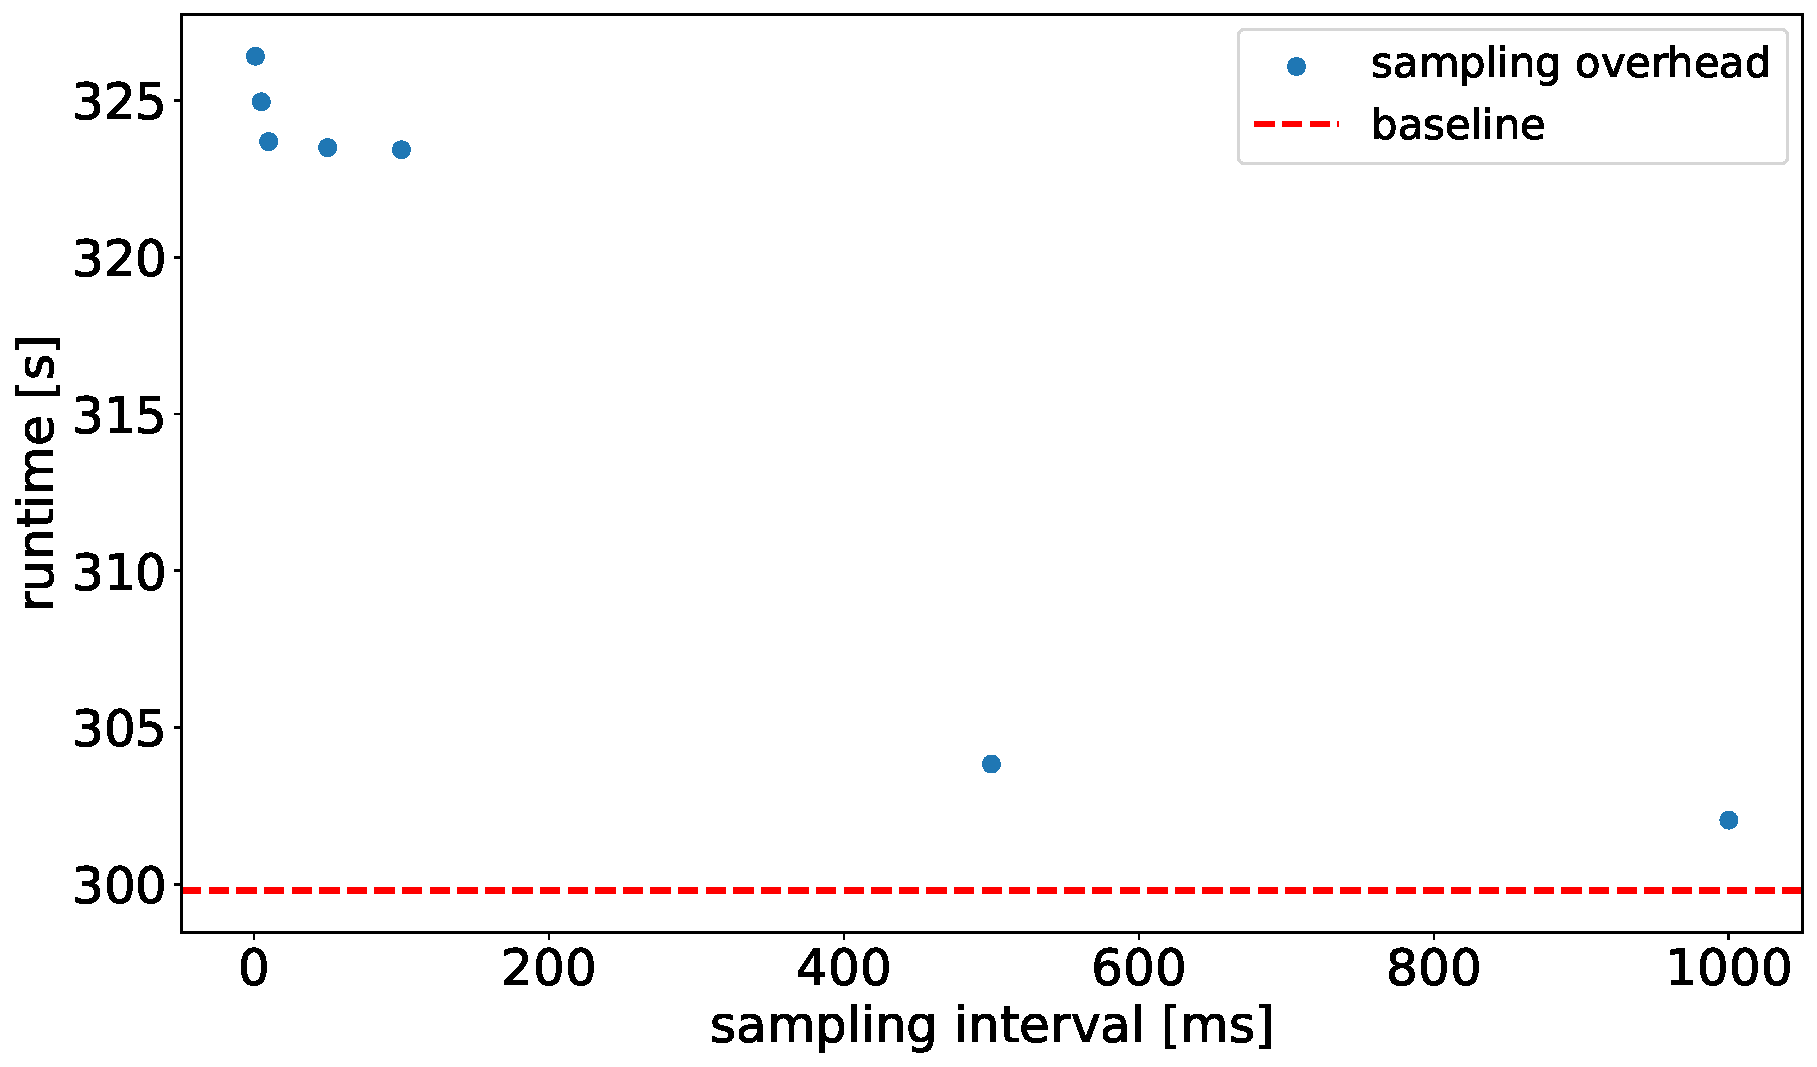
\includegraphics[width=0.8\linewidth]{figures/02_performance_portability/hws_sampling_interval_overhead}
    \caption{%
    The overhead when using the hws library, depends on the specified sampling interval. 
    The red dashed line at the bottom is the baseline version without hws. 
    We can see, that the overhead when using hws is noticeable for smaller sampling intervals. 
    However, increasing the sampling interval also drastically decreases the overhead. 
    }
    \label{fig:hws_overhead}
\end{figure}
\todo{remake plot (new runtimes with more data points)}

% \begin{figure}
%     \centering
    
%     \caption{%
%     The overhead when using the hws library, depends on the specified sampling interval. 
%     The red dashed line at the bottom is the baseline version without hws. 
%     We can see, that the overhead when using hws is noticeable for smaller sampling intervals. 
%     However, increasing the sampling interval also drastically decreases the overhead. 
%     }
%     \label{fig:hws_overhead}
% \end{figure}


\section{What Is Portability?}
\label{sec::portability}

Two main portability types can be meant if we are talking about portability. 
On the one side, binary portability means that I compile my code once, and it runs everywhere. 
On the other side, source code portability means I write portable source code that needs to be recompiled on each new hardware platform. 
Generally, the former is much more challenging to achieve than the latter, and most of the time, some form of \gls{jit} compilation is involved. 
For the remainder of this thesis, if I talk about portability, I mean source code portability. 

The need for portable codes, in general, has been an ongoing problem for many years. 
One of the first portability definitions was already provided in \citeyear{poole_portability_1975} fifty years ago: 
\begin{quotebox}{\citet{poole_portability_1975}}
    Portability is a measure of the ease with which a program can be transferred from one environment to another: If the effort required to move the program is much less than that required to implement it initially, then we say that it is highly portable.
\end{quotebox}
% which was later picked up or slightly modified by other publications~\cite{tanenbaum_guidelines_1978, mooney_bringing_1997}. \todo{cite? more?}

\todo{find more definitions?}

Based on the slight modification of this portability definition from \citet{mooney_bringing_1997}, \citet{sedova_high-performance_2018} devised a formal definition of portability:
\begin{definition}[Portability~\cite{sedova_high-performance_2018}]
An application can be said to be portable if the cost of porting is less than the cost of re-writing:
$$DP = 1 - \left(\frac{C_P}{C_R}\right)$$
where $C_P$ is the cost to port, and $C_R$ is the cost to rewrite the program. 
\end{definition}
A program is completely portable if $DP$ is one, and a positive value indicates that porting a code is more profitable than rewriting it from scratch. 

A more recent definition of portability was created by \citet{pennycook_metric_2016, pennycook_implications_2019} which define portability as: 
\begin{quotebox}{\citet{pennycook_implications_2019}}
    The ability of an application to execute a problem correctly on a given set of platforms.
\end{quotebox}
In contrast to the previous definition, the key part here is that it is not enough for an application to run on different hardware platforms but to produce the correct results on these different platforms. 
An application that runs everywhere but produces wrong results is pointless in a real-world setting. 

\todo{insert ways to fix the portability problem}

\newpage
\subsection{OpenMP -- Open Multi-Processing}

OpenMP (Target Offloading)
\begin{itemize}
    \item first OpenMP specification version 1.0 (C/\cpp) October 1998~\cite{openmp_architecture_review_board_openmp_1998}
    \item first OpenMP specification with target offloading version 4.0 July 2013~\cite{openmp_architecture_review_board_openmp_2013}
    \item current OpenMP specification version 6.0 November 2024~\cite{openmp_architecture_review_board_openmp_2024}
    \item Implementations (Auszug)(\url{https://www.openmp.org/resources/openmp-compilers-tools/})
    \begin{itemize}
        \item AMD
        \item Intel
        \item LLVM
        \item GNU
        \item ARM
        \item NVIDIA
        \item PGI
        \item $\dots$
    \end{itemize}
\end{itemize}


\begin{itemize}
    \item \acrfull{openmp}
    \item pragma based
    \item least invasive; pragmas ignored if no OpenMP capable compiler could be found
    \item but comes also with a runtime library 
    \item originally meant for CPUs only
    \item standardized
    \item uses the fork-join model; initial thread spawns worker threads
    \item uses a custom OpemMP thread pool
    \item task- and loop-parallelism (only latter is used)
\end{itemize}


\begin{advantagebox}
    \begin{itemize}
        \item standardized
        \item supports a wide variety of hardware platforms
        \item non-intrusive and easy-to-use
    \end{itemize}
\end{advantagebox}

\begin{disadvantagebox}
    \begin{itemize}
        \item very high-level, i.e., some optimizations not possible
    \end{itemize}
\end{disadvantagebox}

\newpage
\subsection{CUDA -- Compute Unified Device Architecture}

CUDA
\begin{itemize}
    \item first release of CUDA 1.0 June, 2007~\cite{nvidia_corporation_cuda_2007}
    \item current release of CUDA 12.8 February, 2025~\cite{nvidia_corporation_cuda_2025-1}
    \item the current CUDA programming guide February, 2025~\cite{nvidia_corporation_cuda_2025}
    \item first CUDA version (3.0) deprecating device emulation mode March, 2010~\cite{nvidia_corporation_cuda_2010}
\end{itemize}

\begin{itemize}
    \item \acrfull{cuda}
    \item NVIDIA's own vendor-specific framework
    \item C-like API with custom extensions \code{<<<...>>>}
    \item only for NVIDIA \glspl{gpu}
    \item offload compute kernels from host (i.e., classically \glspl{cpu}) to one or more devices
    \item many vendor-provided, highly optimized libraries available (e.g., cuBLAS, cuSPARSE, cuFFT, $\dots$)
    \item interfaces for C, C++, FORTRAN, Python, Matlab, Java
\end{itemize}

\begin{advantagebox}
    \begin{itemize}
        \item practically, the go-to standard to target \glspl{gpu}
        \item many resources available
        \item high optimization potential
    \end{itemize}
\end{advantagebox}

\begin{disadvantagebox}
    \begin{itemize}
        \item not standardized
        \item only NVIDIA \glspl{gpu}
        \item closed-source proprietary
    \end{itemize}
\end{disadvantagebox}

\newpage
\subsection{HPX -- High Performance ParallelX}
\label{sec:frameworks:hpx}

\begin{quotebox}{\href{https://hpx-docs.stellar-group.org/latest/html/index.html\#what-is-hpx}{HPX Documentation}}
    HPX is a C++ Standard Library for Concurrency and Parallelism. It implements all of the corresponding facilities as defined by the C++ Standard. Additionally, in HPX we implement functionalities proposed as part of the ongoing C++ standardization process. We also extend the C++ Standard APIs to the distributed case. HPX is developed by the STE||AR group.
\end{quotebox}

\acrfull{hpx}~\cite{kaiser_hpx_2020} is high-performance many-task asynchronous tasking library. 
Its development started in 2007~\cite{the_stear_group_history_nodate} with the current version being v1.10.0 from March 2024~\cite{kaiser_stellar-grouphpx_2024}.
Although \gls{hpx} is not standardized where possible, its \gls{api} is closely modeled after the \cpp standard \gls{api}. 

The execution model of \gls{hpx} is based on a task graph that is implicitly built in the source code and later executed asynchronously. 
It implements custom schedulers that also incorporate work-stealing to automatically improve the load-balancing of applications using \gls{hpx}. 
This is especially useful for non-uniform problems that rely on good load balancing. 
\gls{hpx} also supports distributed memory architectures using an \gls{agas} and different accelerators using executors. 
Note that \gls{hpx} only portably incorporates kernel launches in its internal task graph; the actual compute kernels must still be written using other frameworks like \gls{cuda}, \gls{hip}, Kokkos, or SYCL.  
Additionally, \gls{hpx} supports the \cpp{17} standard library parallel algorithms (also see~\autoref{sec:frameworks:stdpar}. 
In the remainder of this thesis, only these standard algorithms are used with \gls{hpx}. 

\todo{mention that parallel algorithms were only implemented after the \cpp draft}

\begin{listing}
    \begin{minted}{cpp}
std::vector<int> indices(N);
std::iota(indices.begin(), indices.end(), 0);

hpx::for_each(hpx::execution::par_unseq, indices.begin(), indices.end(), [&](const int idx) {
    Y[idx] = alpha * X[idx] + Y[idx];
});
    \end{minted}
    \caption{%
    A simple DAXPY example using \gls{hpx} parallel loops.}
    \label{code:hpx_example}
\end{listing}

An example of these \cpp{17} standard parallel algorithms can be seen in \autoref{code:hpx_example}. 
The only difference compared to \autoref{code:stdpar_example} is the usage of the \code{hpx::} namespace qualifiers instead of the \code{std::} ones. 
In this code, the \code{for_each} loop is automatically parallelized across all available \gls{cpu} cores. 


%%% ADVANTAGES AND DISADVANTAGES
\AdvantagesAndDisadvantages{hpx}{
    \item supports algorithms close to \cpp standard
    \item task-based abstraction more suitable for some problems
}{
    \item not standardized
    \item can only launch kernels, other frameworks still \textbf{necessary} to write the actual compute kernels 
}

\newpage
\subsection{OpenCL -- Open Computing Language}

OpenCL:
\begin{itemize}
    \item \enquote{OpenCL is a trademark of Apple Inc. used under license to the Khronos Group Inc}
    \item working group created 2008~\cite{khronos_opencl_working_group_khronos_2008}
    \item first speciifcation published 2009~\cite{munshi_opencl_2009}
    \item current standard OpenCL 3.0 revision 17 October 24, 2024~\cite{khronos_opencl_working_group_opencl_2024}
    \item Implementations OpenCL 3.0 (\url{https://www.khronos.org/conformance/adopters/conformant-products/opencl})
    \begin{itemize}
        \item Intel
        \item Imagination Technologies
        \item QUALCOMM
        \item Google, Inc. 
        \item Software Freedom Conservancy
        \item Arm Limited
        \item NVIDIA
        \item Software in the Public Interest, Inc.
        \item Verisilicon, Inc.
        \item pocl
    \end{itemize}
    \item many more for OpenCL 2.0 (like AMD, Samsung Electronics, etc.)
\end{itemize}

\begin{itemize}
    \item \acrfull{opencl}
    \item standardized
    \item kernels are simple strings $\rightarrow$ easy to manipulate, tedious to use
    \item kernels must be compiled by yourself using OpenCL provided functions
    \item C API
    \item \gls{jit} compiled
    \item programming model/kernel structure close to \gls{cuda}
\end{itemize}

\begin{advantagebox}
    \begin{itemize}
        \item standardized
        \item supports a wide variety of hardware platforms (many implementations)
    \end{itemize}
\end{advantagebox}

\begin{disadvantagebox}
    \begin{itemize}
        \item kernels must be compiled by hand
        \item error prone
        \item some low-level optimizations not possible
    \end{itemize}
\end{disadvantagebox}


\begin{listing}
    \begin{minted}{cpp}
const char* kernel_source = R"KS(
__kernel void saxpy(const double alpha, __global double *X, __global double *X) {
    const int idx = get_global_id(0);
    Y[idx] = alpha * X[idx] + Y[idx];
}
)KS";

cl_platform_id platform;
clGetPlatformIDs(1, &platform, nullptr);
cl_device_id device;
clGetDeviceIDs(platform, CL_DEVICE_TYPE_GPU, 1, &device, nullptr);
cl_context context = clCreateContext(nullptr, 1, &device, nullptr, nullptr, nullptr);
cl_command_queue queue = clCreateCommandQueue(context, device, 0, nullptr);

cl_mem d_X = clCreateBuffer(context, CL_MEM_READ_ONLY | CL_MEM_COPY_HOST_PTR, N * sizeof(double), X, nullptr);
cl_mem d_Y = clCreateBuffer(context, CL_MEM_READ_ONLY | CL_MEM_COPY_HOST_PTR, N * sizeof(double), Y, nullptr);

cl_program program = clCreateProgramWithSource(context, 1, &kernel_source, nullptr, nullptr);
clBuildProgram(program, 1, &device, nullptr, nullptr, nullptr);
cl_kernel kernel = clCreateKernel(program, "saxpy", nullptr);

clSetKernelArg(kernel, 0, sizeof(double), &alpha);
clSetKernelArg(kernel, 1, sizeof(cl_mem), &d_X);
clSetKernelArg(kernel, 2, sizeof(cl_mem), &d_Y);

size_t global_size = N;
clEnqueueNDRangeKernel(queue, kernel, 1, nullptr, &global_size, nullptr, 0, nullptr, nullptr);
clEnqueueReadBuffer(queue, d_C, CL_TRUE, 0, N * sizeof(double), C, 0, nullptr, nullptr);

clReleaseMemObject(d_X); 
clReleaseMemObject(d_Y);
clReleaseKernel(kernel); 
clReleaseProgram(program);
clReleaseCommandQueue(queue); 
clReleaseContext(context);
    \end{minted}
    \caption{%
    SAXPY example using \gls{opencl}.
    }
    \label{code:opencl_example}
\end{listing}
\newpage
\subsection{SYCL}

SYCL:
\begin{itemize}
    \item first provisional specification March 19, 2014~\cite{khronos_sycl_working_group_khronos_2014}
    \item first official release of SYCL 1.2 specification May 11, 2015~\cite{khronos_sycl_working_group_khronos_2015}
    \item current standard SYCL 2020 Rev 9 August 18, 2024~\cite{khronos_sycl_working_group_sycl_2024}
    \item Implementations (\url{https://www.khronos.org/sycl/#sycl-implementations})
    \begin{itemize}
        \item Intel oneAPI \dpcpp/icpx
        \item AdaptiveCpp
        \item triSYCL
        \item neoSYCL
        \item SimSYCL
    \end{itemize}
\end{itemize}

\begin{itemize}
    \item SYCL
    \item standardized
    \item sinlge-source standard \cpp
    \item \cpp API
    \item easy builtin interoperability with backend specific libraries
    \item different ways to express parallelism
    \item programming model/kernel structure close to \gls{cuda} ($\rightarrow$ automatic \gls{cuda} to SYCL migration tools available)
    \item originally tightly coupled with \gls{opencl}
\end{itemize}


\begin{advantagebox}
    \begin{itemize}
        \item standardized
        \item supports a wide variety of hardware platforms
    \end{itemize}
\end{advantagebox}

\begin{disadvantagebox}
    \begin{itemize}
        \item some low-level optimizations not possible directly in SYCL
    \end{itemize}
\end{disadvantagebox}
\newpage
\subsection{Kokkos}

Kokkos:
\begin{itemize}
    \item first release May 2015~\cite{trott_kokkos_2015}
    \item original Kokkos paper 2024~\cite{carter_edwards_kokkos_2014}
    \item please cite~\cite{trott_kokkos_2022}
    \item current release v 4.5.1 December 23, 2024~\cite{noauthor_release_2024}
\end{itemize}

\begin{itemize}
    \item Kokkos
    \item open-source
    \item \cpp API
    \item interoperability with backend specific libraries
    \item different ways to express parallelism
    \item high-level abstractions, making it easier for new programmers
\end{itemize}


\begin{advantagebox}
    \begin{itemize}
        \item supports a wide variety of hardware platforms with different execution spaces
        \item easy-to-use abstractions like execution and memory spaces
    \end{itemize}
\end{advantagebox}

\begin{disadvantagebox}
    \begin{itemize}
        \item not standardized
        \item abstractions different to \gls{cuda} $\rightarrow$ more difficult to translate from existing \gls{cuda} code
        \item some low-level optimizations not possible directly in Kokkos
    \end{itemize}
\end{disadvantagebox}

\begin{listing}
    \begin{minted}{cpp}
Kokkos::View<double*> d_X("X", N);
Kokkos::View<double*> d_Y("Y", N);
Kokkos::deep_copy(d_X, X);
Kokkos::deep_copy(d_Y, Y);

Kokkos::parallel_for("saxpy", N, KOKKOS_LAMBDA(const int idx) {
    d_Y(idx) = alpha * d_X(idx) + d_Y(idx);
});
Kokkos::fence();

Kokkos::deep_copy(Y, d_Y);
    \end{minted}
    \caption{%
    SAXPY example using Kokkos.
    }
    \label{code:kokkos_example}
\end{listing}

\newpage
\subsection{HIP -- Heterogeneous-computing Interface for Portability}

HIP
\begin{itemize}
    \item first public release 0.82.01 March 08, 2016~\cite{advanced_micro_devices_release_2016}
    \item current release 6.3.3 February, 19 2025~\cite{advanced_micro_devices_release_2025}
    \item current HIP documentation~\cite{advanced_micro_devices_hip_nodate}
    \item HIP for CUDA: \enquote{It’s HIP to be Open}~\cite{advanced_micro_devices_its_2016}
\end{itemize}


\begin{itemize}
    \item \acrfull{hip}
    \item AMD's own vendor-specific framework
    \item C-like API with custom extensions \code{<<<...>>>}
    \item only for AMD and NVIDIA \glspl{gpu}
    \item offload compute kernels from host (i.e., classically \glspl{cpu}) to one or more devices
    \item many vendor-provided, highly optimized libraries available (e.g., hipBLAS, hipSPARSE, hipFFT, $\dots$)
    \item in most cases, conversion between \gls{cuda} and \gls{hip} via simple regex possible
    \item NVIDIA \gls{gpu} support via NVIDIA's compiler stack
\end{itemize}

\begin{advantagebox}
    \begin{itemize}
        \item easy to translate from \gls{cuda}
        \item high optimization potential
    \end{itemize}
\end{advantagebox}

\begin{disadvantagebox}
    \begin{itemize}
        \item not standardized
        \item only AMD and NVIDIA \glspl{gpu}
    \end{itemize}
\end{disadvantagebox}

\begin{listing}
    \begin{minted}{cpp}
__global__ void vector_add(const double alpha, const double *X, double *Y, const int N) {
    const int idx = blockDim.x * blockIdx.x + threadIdx.x;
    if(idx < N) Y[idx] = alpha * X[idx] + Y[idx];
}
    
double *d_X, *d_Y;
hipMalloc(&d_X, N * sizeof(double));
hipMalloc(&d_Y, N * sizeof(double));
hipMemcpy(d_X, X, N * sizeof(double), hipMemcpyHostToDevice);
hipMemcpy(d_Y, Y, N * sizeof(double), hipMemcpyHostToDevice);

vector_add<<<(N + 255) / 256, 256>>>(alpha, d_X, d_Y, N);

hipMemcpy(Y, d_Y, N * sizeof(double), hipMemcpyDeviceToHost);
hipFree(d_X);
hipFree(d_Y);
    \end{minted}
    \caption{%
    SAXPY example using \gls{hip}.
    }
    \label{code:hip_example}
\end{listing}
\newpage
\subsection{Standard \cpp -- stdpar}

standard \cpp
\begin{itemize}
    \item \cpp{17} standard~\cite{international_organization_for_standardization_isoiec_2017}
    \item execution policies introduced with \cpp{17} P0024R2~\cite{hoberock_p0024r2_2016}
    \item \code{std::execution::par_unseq} added in \cpp{20} P1001R2~\cite{meredith_p1001r2_2019}
    \item sender and receiver added in \cpp{26}~\cite{dominiak_p2300r10_2024, baker_p3396r0_2024, niebler_p3325r5_2024}
    \item Implementations:
    \begin{itemize}
        \item GNU GCC + TBB
        \item NVIDIA nvhpc
        \item rocstdpar
        \item AdaptiveCpp
        \item \dpcpp/icpx
    \end{itemize}
\end{itemize}


\begin{itemize}
    \item Standard \cpp
    \item direct part of the \cpp{17} standard
    \item although standard \cpp no all \cpp features allowed inside kernels
    \item parallelization can easily be enabled/disabled using the respective execution policy
\end{itemize}


\begin{advantagebox}
    \begin{itemize}
        \item standardized
        \item supports a wide variety of hardware platforms
        \item extremely easy-to-use if already familiar with \cpp standard algorithms
    \end{itemize}
\end{advantagebox}

\begin{disadvantagebox}
    \begin{itemize}
        \item very high-level, i.e., some optimizations not possible
    \end{itemize}
\end{disadvantagebox}


Other Frameworks:
\begin{itemize}
    \item OpenACC
    \begin{itemize}
        \item first specification November 2011~\cite{openacc_standard_openacc_2011}
        \item first or one of the first OpenACC papers 2012~\cite{hutchison_openacc_2012}
        \item current specification November 2022~\cite{openacc_standard_openacc_2022}
        \item Implementations (\url{https://www.openacc.org/tools})
        \begin{itemize}
            \item HPE Cray Compiler Environment (CCE): OpenACC deprecated since CCE 10.0.0 for C and C++ as of 7 May 2020 (\url{https://support.hpe.com/hpesc/public/docDisplay?docId=a00113907en_us&page=OpenACC_Use.html}, \url{https://support.hpe.com/hpesc/public/docDisplay?docId=a00115296en_us&page=About_the_Cray_Fortran_Reference_Manual.html})
            \item NVIDIA
            \item GCC (\url{https://gcc.gnu.org/wiki/OpenACC})
            \item Omni Compiler Project (\url{https://omni-compiler.org/})
            \item OpenHU (\url{https://github.com/uhhpctools/openuh})
            \item OpenARC (\url{https://github.com/swiftcurrent2018/openarc})
            \item RoseACC (\url{https://github.com/laudarch/RoseACC-workspace})
        \end{itemize}
    \end{itemize}
    
    \item RAJA:
    \begin{itemize}
        \item first release v0.1.0 June 22, 2016~\cite{llnl_release_2016}
        \item first publication 2019~\cite{beckingsale_raja_2019}
        \item current release v2024.07.0 July 24, 2024~\cite{llnl_release_2024}
    \end{itemize}

    \item thrust
    \begin{itemize}
        \item algorithms for NVIDIA GPU and multi-core CPU~\cite{bell_thrust_2012}
        \item first thrust release 1.0.0 June, 2009~\cite{nvidia_corporation_thrust_2009}
        \item current thrust release under the CUDA \cpp Core Libraries 2.8.0 March 03, 2025~\cite{cccl_development_team_release_2023}
    \end{itemize}

    \item Charm++
    \begin{itemize}
        \item GPU Manager library and Hybrid API (HAPI)
        \item source repo~\cite{kale_uiuc-pplcharm_2021}
        \item first release and paper October 1993~\cite{kale_charm_1993}
        \item added support for GPUs~\cite{wesolowski_application_2008}
        \item current release v8.0.0 June 4, 2024~\cite{noauthor_release_2024}
    \end{itemize}

    \item Legion
    \begin{itemize}
        \item \enquote{Legion is a data-centric parallel programming system for writing portable high-performance programs targeted at distributed heterogeneous architectures.}
        \item initial paper including GPU support November, 2012~\cite{bauer_legion_2012}
        \item current release 24.12.0, December 20, 2024~\cite{stanford_release_2024}
    \end{itemize}

    \item Domain-Specific Languages (DSLs)
\end{itemize}

\newpage

\begin{table}[]
    \newcommand{\supported}{\textcolor{ForestGreen}{\faCheckCircle}}
    \newcommand{\partialsupported}{\textcolor{BurntOrange}{\faCheckCircle}}
    \newcommand{\unsupported}{\textcolor{Red}{\faTimesCircle}}
    \centering
    \begin{tblr}{colspec = {Q[l,m] *{6}{X[c,m]}},
                 row{1,2} = {font=\bfseries, bg=gray!50},
                 row{odd[2]} = {bg=gray!25},
                 rowsep=4pt
                 }
        \toprule
                      & \SetCell[c=3]{c}\glspl{cpu} &&             & \SetCell[c=3]{c}\glspl{gpu} &&                            \\
                      & x86\_64      & POWER9       & ARM          & NVIDIA            & AMD               & Intel             \\\midrule
        OpenMP        & \supported   & \supported   & \supported   & \supported        & \supported        & \supported        \\
        CUDA          & \unsupported & \unsupported & \unsupported & \supported        & \unsupported      & \unsupported      \\
        HPX           & \supported   & \supported   & \supported   & \partialsupported & \partialsupported & \partialsupported \\
        OpenCL        & \supported   & \supported   & \supported   & \supported        & \supported        & \supported        \\
        SYCL          & \supported   & \supported   & \supported   & \supported        & \supported        & \supported        \\
        Kokkos        & \supported   & \supported   & \supported   & \supported        & \supported        & \supported        \\
        HIP           & \unsupported & \unsupported & \unsupported & \supported        & \supported        & \unsupported      \\
        Standard \cpp & \supported   & \supported   & \supported   & \supported        & \supported        & \supported        \\
        \bottomrule
    \end{tblr}
    \caption{%
    Either we can use two categories, simply splitting the hardware platforms in \glspl{cpu} and \glspl{gpu}, or split it into more fine-grain categories like different \gls{cpu} and \gls{gpu} architectures. 
    Additional, other hardware platforms inside these categories, e.g., RISC-V \glspl{cpu} or ARM \glspl{gpu} or even completely new categories like \glspl{fpga} or \glspl{tpu} are also possible. 
    For \gls{hpx}, \glspl{gpu} are supported via executors, but the actual compute kernels must be written using another framework like \gls{cuda}, \gls{hip}, SYCL, or Kokkos.
    Note that for the standardized frameworks, it can happen that no single implementation supports all hardware platforms, but only a mixture does. 
    }
    \label{tab:portability_categories}
\end{table}


\begin{table}[]
    \centering
    \begin{tblr}{colspec = {Q[l,m] Q[l,m] Q[l,m] Q[l,m] Q[l,m] Q[l,m]},
                 row{1} = {font=\bfseries, bg=gray!50},
                 row{odd[2]} = {bg=gray!25},
                 rowsep=4pt
                 }
        \toprule
        CUDA             & HIP              & OpenCL            & SYCL              & Kokkos                    & OpenMP \\\midrule
        thread           & thread           & work-item         & work-item         & thread                    & thread \\
        warp             & wavefront        & sub-group         & sub-group         & --                        & -- \\
        {thread\\block}  & {thread\\block}  & work-group        & work-group        & team                      & team \\
        grid             & grid             & nd-range          & nd-range          & league                    & league \\
        register         & register         & {private\\memory} & {private\\memory} & register                  & register \\
        {shared\\memory} & {shared\\memory} & {local\\memory}   & {local\\memory}   & {scratchpad\\memory}      & shared \\
        {global\\memory} & {global\\memory} & {global\\memory}  & {global\\memory}  & \makecell{memory\\spaces} & -- \\
        \bottomrule
    \end{tblr}
    \caption{%
    The different naming conventions for the different portability languages and frameworks. 
    Since my greatest focus lies on SYCL, I will use its naming convention going forward. 
    For Standard \cpp, these notations do not apply since the \cpp standard has no notion of the underlying hardware because it is only defined on an abstract state machine. 
    }
    \label{tab:portability_naming}
\end{table}


\section{Performance + Portability}


Until now, I looked at performance and portability separately which is OK since sometimes one is only interested in one of these aspects. 
One may know that the code will only ever be executed on one specific hardware platform, and it is important to achieve the best performance possible down to the assembly level. 
On the other hand, for some, it may be enough to write code that can be executed everywhere but that must not necessarily be performant. 
However, for many achieving a combination of both is also important: writing code that can be executed on a variety of different hardware, without the need to re-implement everything from scratch again if the hardware changes, but that also achieves reasonable performance on all hardware. 
By reasonable here I mean that it achieves a high enough fraction of the possible achievable performance. 
It should be clear that it is extremely difficult or even impossible to achieve the same performance with code that can run on all \glspl{gpu} and \glspl{cpu} there are compared to highly optimized vendor-specific solutions that may even be implemented by the vendors themselves with special closed-source knowledge of the underlying hardware. 

Assessing performance portability is an ongoing research topic. 
Over the years, many definitions emerged starting with more informal definitions of performance portability. 
Note that the following definitions aren't exhaustive but only serve as examples.


%%% QUOTES - informal Performance Portability definitions


In 2013 in their original Kokkos paper \citeauthor{edwards_kokkos_2013} defined performance portability as:
\begin{quotebox}{\citet{edwards_kokkos_2013}}
    Our performance portability objective is to maximize the amount of user code that can be compiled for diverse devices and obtain the same (or nearly the same) performance as a variant of the code that is written specifically for that device.
\end{quotebox}
While this definition was already quite good, the problem is that \enquote{\textit{nearly the same}} can and will be interpreted differently by different people. 
Therefore, this definition is not feasible to use as an object performance portability metric.

In 2014 \citeauthor{kunkel_performance_2014} defined performance portability as:
\begin{quotebox}{\citet{kunkel_performance_2014}}
    A code is performance portable if it can achieve a similar fraction of peak hardware performance on a range of different target architectures.
\end{quotebox}
As with the quote from \citeauthor{edwards_kokkos_2013} the problem is the objectivity of the definition namely how big the \enquote{\textit{similar fraction of}} should be. 
Although \citeauthor{kunkel_performance_2014} stated that for them it is \SI{20}{\percent} of the \enquote{best achievable performance} with respect to a hand-optimized native implementation, another person could argue that it should be \SI{15}{\percent} or \SI{25}{\percent} making this metric also highly subjective. 

In 2016 \citet{larkin_performance_2016} defined performance portability as:
\begin{quotebox}{\citet{larkin_performance_2016}}
    The same source code will run productively on a variety of different architectures.
\end{quotebox}
Again, \enquote{\textit{productively}} is highly subjective not only in a performance but also in a portable way. 
This definition can include that maintaining custom code paths for better performance may be ok as long as it is not too much work. 

Also in 2016, the \gls{doe} conducted a meeting \cite{neely_doe_2016} specifically regarding performance portability. 
There, a few attendees were asked to define performance portability in their own words:
\begin{quotebox}{Rob Neely~\cite{neely_doe_2016}}
    For purposes of this meeting, it is the ability to run an application with acceptable performance across KNL and GPU-based systems with a single version of source code.
\end{quotebox}
\begin{quotebox}{Simon Pennycook~\cite{neely_doe_2016}}
    An application is performance portable if it achieves a consistent level of performance (e.g. defined by execution time or other figure of merit, not percentage of peak flops across platforms relative to the best known implementation on each platform.
\end{quotebox}
\begin{quotebox}{Adrian Pope, Vitali Morozov~\cite{neely_doe_2016}}
    Hard portability = no code changes and no tuning. Software portability = simple code mods with no algorithmic changes. Non-portable = algorithmic changes.
\end{quotebox}
\begin{quotebox}{David Richards~\cite{neely_doe_2016}}
    A code is performance portable when the application team says its performance portable!
\end{quotebox}

At the end of the \gls{doe} meeting, the attendees also created a working definition trying to incorporate the above definitions into one: 
\begin{quotebox}{\gls{doe} Working Definition~\cite{doe_meeting_attendees_definition_nodate}}
    An application is performance portable if it achieves a consistent ratio of the actual time to solution to either the best-known or the theoretical best time to solution on each platform with minimal platform specific code required.
\end{quotebox} % https://performanceportability.org/perfport/definition/

As with all other previous definitions, all of these quotes contain some objective part in one way or another.
However, to discuss performance portability objectively, these subjective definitions can not be used if it is expected that everyone should agree on the same values. 


%%% formal Performance Portability definitions


Therefore, the first objective performance portability metric was introduced by \citeauthor{pennycook_implications_2019} at the end of 2016 published on arXiv~\cite{pennycook_metric_2016}, and finally submitted as a full paper at the beginning of 2017~\cite{pennycook_implications_2019}. 
It was the first formal definition that can be used to assess the performance portability of an application objectively.

\begin{definition}[Performance Portability \pp~(Pennycook et al.~\cite{pennycook_implications_2019})]\label{def:pp}
    Given a problem $\mathbf{p}$ which is solved by an application $\mathbf{a}$ and a set of platforms $\mathbf{H}$, the performance portability metric \pp is defined as:

    \[ \pp(a, p, H) = 
        \begin{cases}
            \frac{\abs{H}}{\sum\limits_{i \in H} \frac{1}{e_i(a, p)}} & \text{if }i\text{ is supported } \forall i \in H \\
            0                                                         & \text{otherwise}
        \end{cases} 
    \]

    where $\mathbf{e_i}$ is the performance efficiency of $\mathbf{a}$ solving $\mathbf{p}$ on platform $\mathbf{i \in H}$.
\end{definition}

Therefore, the performance portability metric \pp is the harmonic mean over the performance efficiency of an application solving a specific problem on all tested hardware platforms. 
The only difference to the harmonic mean is that \pp is also defined if the input data, i.e., the performance efficiency, includes a $0$. 
The \pp metric has the nice property that, per construction, it is in the interval $\interval{0}{1}$ where $0$ means the application did not run on all hardware platforms and $1$ means the best possible performance on all hardware platforms. 

Note that \pp heavily emphasizes the \textit{portability} aspect of performance portability: If only one hardware platform is not supported the result of \pp will directly be $0$ regardless of the performance on all other hardware platforms. 
Depending on your target audience, this property of \pp may be desirable or not. 

\todo{Marowka's Kritik aufzählen}
\cite{marowka_toward_2021, marowka_reformulation_2022, marowka_comparison_2023, marowka_portability_2024, marowka_inorrect_2024}

\todo{highlight \textbf{same architecture class}}

\begin{definition}[Performance Portability \mpp~(\citet{marowka_comparison_2023})]\label{def:mpp}
    Given a problem $\mathbf{p}$ which is solved by an application $\mathbf{a}$ and a set of supported platforms $\mathbf{S \subseteq H}$ from the same architecture class, the performance portability metric $\overline{\pp}$ is defined as:

    \[ \mpp(a, p, S, H) = 
        \begin{cases}
            \frac{\sum\limits_{i \in S} e_i(a, p)}{\abs{S}} & \text{if }\abs{S} > 0 \\
            0                                               & \text{otherwise}
        \end{cases} 
    \]

    where $S \coloneqq \{ i \in H | e_i(a, p) > 0 \}$ and $\mathbf{e_i}$ is the performance efficiency of $\mathbf{a}$ solving $\mathbf{p}$ on platform $\mathbf{i \in H}$.
\end{definition}

In contrast to \pp, \mpp is defined as the normal mean across all \textbf{supported} platforms. 
The value of \mpp is $0$ if and only if \textbf{no} hardware platform in $\mathbf{H}$ is supported by the current application $\mathbf{a}$. 
This also shows us the main emphasis of \mpp in contrast to \pp: For \mpp the \textit{performance} aspect of performance portability is heavily emphasized since an application that does not run on all hardware platforms is not penalized as with \pp. 

\todo{way more complex metric}
As a response to \citeauthor{marowka_comparison_2023} critic to their performance portability metric \pp, \citet{pennycook_revisiting_2021} updated their metric to include \todo{was kam dazu?}


\citet{harrell_effective_2018} extended the performance portability even further to an \textit{effective performance portability} that does not only include the above-discussed performance portability but also the productivity, i.e., the effort a programmer has to make to achieve said performance portability. 
This metric also penalizes frameworks that achieve good performance portability but only by drastically increasing the programmer's effort, e.g., introducing special code paths for some hardware platforms. 
However, in the remainder of this thesis, I will mainly focus on \textit{performance portability} only. \todo{Begründung?}


\todo{order}
%%% performance efficiency metrics


Both formal performance portability definitions---\pp and \mpp---use a \textit{performance efficiency} $\mathbf{e_i(a, p)}$ in their definition which describes the relation between the achieved performance with respect to some proven expected performance. 
In general, two different definitions defining the performance efficiency of an application $\mathbf{a}$ solving problem $\mathbf{p}$ on the hardware $\mathbf{i \in H}$ are used. 

\begin{definition}[Architectural Efficiency]\label{def:arch_eff}
    The achieved performance as a fraction of the \enquote{peak} theoretical hardware performance, being it the achieved \si{\flop\per\second} or memory bandwidth.
\end{definition}

The \textit{architectural efficiency}

\begin{definition}[Application Efficiency~(\citet{satish_can_2012})]\label{def:app_eff}
    The achieved performance as a fraction of the \enquote{best} observed performance. 
\end{definition}

The \textit{application efficiency}

\todo{3-P challenge: performance, portability, and productivity}

\subsection{Examples}

\begin{table}[]
    \centering
    \begin{tabular}{c|C{1.5cm}|C{1.5cm}|C{1.5cm}|C{1.5cm}}
        \multirow{2}{*}{Platform Set $\mathbf{H}$} & \multicolumn{2}{c|}{Application 1}     & \multicolumn{2}{c}{Application 2}     \\
                                                   & Arch. Eff.        & App. Eff.          & Arch. Eff.        & App. Eff.         \\\midrule
        A                                          & \SI{40}{\percent} & \SI{100}{\percent} & \SI{30}{\percent} & \SI{90}{\percent} \\
        B                                          & \SI{20}{\percent} & \SI{85}{\percent}  & \SI{30}{\percent} & \SI{85}{\percent} \\
        C                                          & \SI{15}{\percent} & \SI{60}{\percent}  & \SI{15}{\percent} & \SI{40}{\percent} \\
        D                                          & --                & --                 & \SI{40}{\percent} & \SI{70}{\percent}
    \end{tabular}
    \caption{%
    Example architectural (arch. eff.) and application (app. eff.) efficiencies for two example applications on four different hardware platforms. 
    Note that the application 1 does not support the architecture D. 
    }
    \label{tab:platforms_example}
\end{table}

\todo{update table}
\begin{table}[]
    % https://www.programiz.com/online-compiler/0apVuVZDNe38e
    \centering
    \begin{tabular}{c|rrrr}
        
        Application 1           & \multicolumn{2}{c}{$\pp(a, p, H)$}          & \multicolumn{2}{c}{$\mpp(a, p, S, H)$}   \\
        Subsets of $\mathbf{H}$ & Arch. Eff.           & App. Eff.            & Arch. Eff.        & App. Eff.            \\\midrule
        \{ A \}                 & \SI{40}{\percent}    & \SI{100}{\percent}   & \SI{40}{\percent} & \SI{100}{\percent}    \\
        \{ A, B \}              & \SI{26.67}{\percent} & \SI{91.89}{\percent} & \SI{30}{\percent} & \SI{92.5}{\percent}  \\
        \{ A, B, C \}           & \SI{21.18}{\percent} & \SI{78.06}{\percent} & \SI{25}{\percent} & \SI{81.67}{\percent} \\
        \{ A, B, C, D \}        & \SI{0.0}{\percent}   & \SI{0.0}{\percent}   & \SI{25}{\percent} & \SI{81.67}{\percent} 
    \end{tabular}
    \caption{%
    The calculated values for \pp and \mpp for application 1 using different subsets of $\mathbf{H}$ and the performance efficiencies given in \autoref{tab:platforms_example}. 
    This example shows the differences between \pp and \mpp if the unsupported hardware platform D is added to the platform set $\mathbf{H}$.
    }
    \label{tab:pp_app_1_example}
\end{table}

\begin{table}[]
    % https://www.programiz.com/online-compiler/0apVuVZDNe38e
    \centering
    \begin{tabular}{c|rrrr}
        Application 2           & \multicolumn{2}{c}{$\pp(a, p, H)$}          & \multicolumn{2}{c}{$\mpp(a, p, S, H)$}      \\
        Subsets of $\mathbf{H}$ & Arch. Eff.           & App. Eff.            & Arch. Eff.           & App. Eff.            \\\midrule
        \{ A \}                 & \SI{30}{\percent}    & \SI{90}{\percent}    & \SI{30}{\percent}    & \SI{90}{\percent}    \\
        \{ A, B \}              & \SI{30}{\percent}    & \SI{87.43}{\percent} & \SI{30}{\percent}    & \SI{87.5}{\percent}  \\
        \{ A, B, C \}           & \SI{25}{\percent}    & \SI{62.66}{\percent} & \SI{25}{\percent}    & \SI{71.67}{\percent} \\
        \{ A, B, C, D \}        & \SI{25.26}{\percent} & \SI{64.35}{\percent} & \SI{28.75}{\percent} & \SI{71.25}{\percent}
    \end{tabular}
    \caption{%
    The calculated values for \pp and \mpp for application 2 using different subsets of $\mathbf{H}$ and the performance efficiencies given in \autoref{tab:platforms_example}. 
    This example shows the differences between \pp and \mpp if all hardware platforms in the platform set $\mathbf{H}$ are supported.
    }
    \label{tab:pp_app_2_example}
\end{table}
\subsection{Visualization of Performance Portability}

\citet{sewall_interpreting_2020} 
different visualization strategies:
\begin{itemize}
    \item Box Plots: obscures the "did not run" case (large boxes); no number of supported platforms; only median to compare in case of "did not run" (boxes cover whole range)
    \item Histograms: distribution of bins ("did not run" must be own bin; how many bins?); areas of low density $\rightarrow$ difficult to "see" the distribution
    \item Probability Density Function: primary problem choosing a good kernel bandwidth; PP sparse and uneven distributed data $\rightarrow$ no fixed bandwidth guaranteed to yield satisfactory results $\rightarrow$ adaptive methods; problems on [0, 1] boundaries $\rightarrow$ there may be many points there for PP making this problem even worse; but better than Histograms (better tendencies; less crowded bars)
    \item Violin Plots: a combination of kernel density estimation and Box Plots

    % Impact of Platform Selection
    \item plotting \pp against $\mathcal{H}$ $\rightarrow$ other paper \cite{deakin_performance_2019}
    \item Efficiency Cascade Plots + Platform Charts: minimum efficiency and H $\rightarrow$ remove platform with minimum efficiency and start again; independent for each application; platform sets at the bottom may not be the same for each application; monotonic decreasing
\end{itemize}

\todo{Plot script anpassen und für mich unnötiges Zeug rauswerfen.}
\begin{figure}
    \centering
    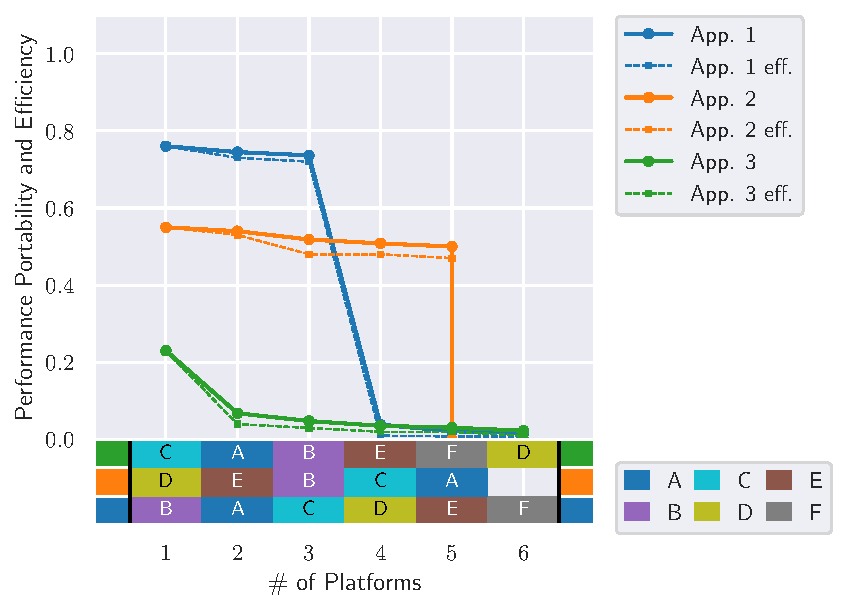
\includegraphics[width=\linewidth]{figures/02_performance_portability/example_diss_eff_cascade.pdf}
    \caption{%
    An example visualization of the performance efficiencies of \autoref{tab:platforms_example} and performance portability metrics of the two example applications from \autoref{tab:pp_app_1_example} and \autoref{tab:pp_app_2_example} as proposed by \citet{sewall_interpreting_2020}. 
    TODO: further description, falsch für \mpp?
    }
    \label{fig:pp-example-visualization}
\end{figure}

\newpage
\cite{pennycook_implications_2019}

\todo{irgendwie folgende Punkte noch unterbringen}
\begin{itemize}
    \item genaue Beschreibung von "platform": a specific hardware, OS, runtime system, etc. $\rightarrow$ hier \textbf{hardware}
    \item genaue Beschreibung von "application": software, die auf ihre Korrektheit überprüft werden kann $\rightarrow$ portability nicht nur definieren als "kann darauf laufen" sondern zusätzlich such "produziert korrektes resultat
    \item productivity schwierig zu messen/nicht objektiv, da sehr von skillset des jeweiligen Programmierers abhängig
    \item also formal Definition vor Pennycook rein?: Performance Portability on EARTH: A Case Study Across Several Parallel Architectures,
    \item arch: kann 100\% peak sein aber trotzdem nicht performant (z.B. bandwidth bound); z.B. via Roofline Model
    \item app: best known != best possible
    \item efficiency: 1 best possible; the lower, the worse
    \item 5 Kriterien an \pp aufnehmen?
    \item arch vs app : was rauslesen wenn eines klein, anderes groß
\end{itemize}

Performance Definition
\begin{quotebox}{\cite{pennycook_implications_2019}}
    Any measurable property of an application’s correct execution of a problem on a platform.
\end{quotebox}

Portability Definition
\begin{quotebox}{\cite{pennycook_implications_2019}}
    The ability of an application to execute a problem correctly on a given set of platforms.
\end{quotebox}

Performance Portability muss folgendes haben: 
\begin{itemize}
    \item beide obigen Definitionen nicht verletzen
    \item objektiv messbar, quantifizierbar und vergleichbar sein
\end{itemize}

Ihre Definition:
\begin{quotebox}{\cite{pennycook_implications_2019}}
    A measurement of an application’s performance efficiency for a given problem that can be executed correctly on all platforms in a given set.
\end{quotebox}


Current Problems in Performance Portability:
\begin{itemize}
    \item "abstraction and irreducible complexity": best Performance ohne spezialisierte Code-Pfade $\rightarrow$ hohe Abstraktionsebene, automatische Code-Generierung für performance
    \item "(still) no silver bullet": 
\end{itemize}

Approaches to Code Spezialization
\begin{itemize}
    \item libraries
    \item DSL
    \item Portability and Productivity Frameworks
    \item Autotuning
    \item Application-specific abstractions
    \item performance portable algorithms

    \item we use frameworks + autotuning in the remainder of this work
    \item for more information on vor- und nachteile see paper \cite{pennycook_implications_2019}
\end{itemize}

Criteria: (verbatim quote)
\begin{enumerate}
    \item Be measured specific to a set of platforms of interest $\mathcal{H}$.
    \item Be independent of the absolute performance across $\mathcal{H}$.
    \item Be zero if a platform in $\mathcal{H}$ is unsupported, and approach zero as the performance of platforms in $\mathcal{H}$ approaches zero. 
    \item Increase if performance increases on any platform in $\mathcal{H}$.
    \item Be directly proportional to the sum of scores across $\mathcal{H}$.
\end{enumerate}

\newpage
\cite{marowka_toward_2021}

\begin{itemize}
    \item Hauptproblem: harmonic mean
    \item Criterion 5 verletzt
    \item Criterion 3 (0 wenn cannot run) only a constrained because of the harmonic mean being undefined for $0$ values
    \item \pp to broad; research results are therefore unrealistic or biased
    \item geometric + harmonic mean won't work, arithmetic does 
    \item new platform, wobei das Verhältnis der Summe aller scores ($e_i$) gleich bleibt, ändert das Verhältnis von \pp
    \item Hat Probleme mit $0$ wenn nicht unterstützt
    \item harmonic mean tends to track more the lower values $\rightarrow$ in general smaller \pp than \mpp values
    \item calculate values for, e.g., CPUs and GPUs separately
    \item if we have no baseline (except a time that would be included in \pp), exclude it from \mpp
\end{itemize}

erste Definition:
\begin{definition}[Performance Portability \mpp~(\citet{marowka_comparison_2023})]\label{def:mpp}
    Given a problem $\mathbf{p}$ which is solved by an application $\mathbf{a}$ and a set of supported platforms $\mathbf{H}$ from \textbf{the same architecture class}, the performance portability metric $\overline{\pp}$ is defined as:

    \[ \mpp(a, p, H) = 
        \begin{cases}
            \frac{\sum\limits_{i \in H} e_i(a, p)}{\abs{H}} & \text{if }i\text{ is supported }\forall i \in H \\
            \textit{not applicable}                         & \text{otherwise}
        \end{cases} 
    \]

    where $\mathbf{e_i}$ is the performance efficiency of $\mathbf{a}$ solving $\mathbf{p}$ on platform $\mathbf{i \in H}$.
\end{definition}
$\rightarrow$ update of criterion 3 with \textit{not applicable}

\newpage
\cite{marowka_reformulation_2022}
$\rightarrow$ extended paper from \cite{marowka_toward_2021}

\begin{itemize}
    \item \enquote{Just because there is no implementation for a single architecture in |H|, for whatever reason, to conclude that the application is not at all portable and its = 0\% is unrealistic.}
    \item Observation 1: Verhältnis wird nicht gewahrt, wenn man eine platform hinzufügt
    \item Observation 2: Probleme mit application efficiency also baseline (ein $a$ nehmen, das schon in \pp mit drin ist)
    \item Observation 3: contradictions Aufgrund von 0
    \item Observation 4: problem if $0$
    \item Observation 5: Probleme, wenn man komplett unterschiedliche Architekturen anschaut (CPU vs GPU bspw.)
    \item Observation 6: do not change between baselines (may result in efficiencies greater 1 but that mahct nichts aus)
    \item \pp GENERELL abhängig von der input Größe
    \item arch vs app efficiency: bei einem bleiben!; peak vs roofling: peak schlechtere Zahlen, aber einheitlich, roofline "fairer" aber uneinheitlich; app eff: NUR wenn es eine optimierte Fassung für alle hardware gibt, nicht in \pp pder \mpp mit aufnehmen! \\$\rightarrow$ app nehmen wenn so eine baseline exisitiert, sonst arch 
\end{itemize}

Redefinition Problem: 
\begin{quotebox}
    computational problem is a collection of questions that computers might be able to solve
\end{quotebox}

application $\rightarrow$ case-study application
\begin{quotebox}
    A given case-study application is a problem that is computationally solved by an algorithm for a given set of input parameters, which is implemented in a performance portability framework, and which is mapped onto a back-end programming model and executed on a given architecture.
\end{quotebox}

Usage Guidelines (copied verbatim) $\rightarrow$ schreiben, was wir davon in späteren Kapiteln einhalten?
\begin{itemize}
    \item It is advisable not to calculate the value of \mpp for platforms of different architecture classes together, such as CPUs and GPUs. If that is what the evaluator is looking for, then it is advisable to present the scores of each architecture class separately.
    \item It is preferable to use the architectural efficiency approach instead of the application efficiency approach.
    \item It is advisable, when using the application efficiency approach, to choose the performance of a low-level, nonportable, and well-optimized implementation as the performance baseline and not to include its score in calculating \mpp.
    \item It is advisable, when using the architectural efficiency approach, to choose theoretical peak performance as the performance baseline.
    \item It is advisable not to include outlier results in calculating \mpp.
    \item It is advisable to include platforms from various vendors in the set of platforms H.
    \item It is advisable that the set of platforms H be as large as possible.
    \item It is advisable that every implementation of the case-study application use the same input parameters, implement the same algorithm, and be compiled by the same compiler and backend compiler.
\end{itemize}

% https://www.digit.in/features/apps/rainbows-unicorns-and-performance-portability-34524.html


\newpage
\cite{pennycook_revisiting_2021}

weitere Kritik: \cite{yokota_beginners_2018, bertoni_performance_2020, siklosi_heterogeneous_2018}

Criteria explained:
\begin{enumerate}
    \item results must be tied to a set of platforms in order for the results to be useful; es ist eben interessant \pp auf unterschiedlicher Hardware (CPUs und GPUs) gemeinsam zu betrachten
    \item differences in the capabilities of $H$ should not bias the results
    \item $0$ als "did not run" macht es vergleichbarer und intuitiver, das sich schlechte Performance der $0$ annähert
    \item encourage users to improve performance across all platforms of interest
    \item original goal \enquote{that comparisons of performance portability reflect comparisons of performance} $\rightarrow$ flaw lies within the criterion and \textbf{not} the formula $\rightarrow$ outliers shouldn't artificially inflate the \pp score $\rightarrow$ after tests, criterion should be discarded
\end{enumerate}

revised criteria:
\begin{enumerate}
    \item Be measured specific to a set of platforms of interest H.
    \item Be independent of the absolute performance of each platform in H.
    \item 
    \begin{enumerate}
        \item Take a numeric value for any set of platforms H.
        \item Be zero if any platform does not run; go to zero as performance on any platform in H goes to zero.
    \end{enumerate}
    \item Increase or decrease if performance increases or decreases on any platform in H, respectively.
\end{enumerate}

Advanced formula: extending \pp to all platforms in H \textbf{executing all problems in P}:

\[ \pp(a, \mathcal{P}, H) = 
        \begin{cases}
            \frac{\abs{\mathcal{P}}\times\abs{H}}{\sum\limits_{p \in \mathcal{P}}\sum\limits_{i \in H} \frac{\Lambda_{i, p}}{\lambda_{i, p}}} & \text{if }\forall i \in \abs{H}\text{ and }\forall p \in \abs{\mathcal{P}}, \lambda_{i, p} \neq 0 \\
            0                         & \text{otherwise}
        \end{cases} 
    \]

\begin{itemize}
    \item do not remove outliers $\rightarrow$ WHAT is a outlier? Maybe outliers reflect the way an application is written?
    \item hergeleitet von "first level principles" $\rightarrow$ \pp soll dadurch interpretierbarer werden
    \item \pp und \mpp: \enquote{alternative weightings of the same underlying summation} $\rightarrow$ weighting by $\frac{\Lambda_i}{\lambda_i}$  vs $\frac{\lambda_i}{\Lambda_i}$
    \item \enquote{\mpp reflects the aggregate throughput that an application would achieve when distributed across H, rather than the aggregate throughput that it should achieve.}
    \item new formula: average over averages $\rightarrow$ information for specific problem lost, but good for summarizing
    \item \enquote{Recall that \pp represents the maximum amount of work when all platforms execute for the same amount of time}
\end{itemize}



\newpage
\cite{marowka_comparison_2023}

\begin{itemize}
    \item versteht nicht, wieso einfach Criterion 5 entfernt wurde
    \item immer noch der Meinung, dass $0$ keinen Sinn ergibt
    \item $\rightarrow$ only include platforms that are supported in \mpp; "not applicable" changed to $0$ such that only numeric values are present
\end{itemize}

Revised criteria for \mpp with $S \in H$
\begin{enumerate}
    \item measured specific to a set of platforms of interest S;
    \item independent of the absolute performance across S;
    \item zero if none of the platforms is supported;
    \item increasing or decreasing if performance increases or decreases on any platform in S;
    \item directly proportional to the sum of scores across S.
\end{enumerate}

neue Formel:
\[ \mpp(a, p, H) = 
        \begin{cases}
            \frac{\sum\limits_{i \in S} e_i(a, p)}{\abs{S}} & \text{if }\abs{S} > 0 \\
            0                         & \text{otherwise}
        \end{cases} 
\]
where $S \coloneqq \{ i \in H | e_i(a, p) > 0 \}$

\begin{itemize}
    \item \pp Hauptproblem: tracks low values $\rightarrow$ architectural efficiency typically on the low side (mostly for CPUs) $\rightarrow$ \pp doesn't really track improvements
    \item proportionality one of the main goals $\rightarrow$ removed from \pp $\rightarrow$ why?
    \item not comparable
    
\end{itemize}

Problems with \cite{smith_characterizing_1988} (copied):
\begin{enumerate}
    \item Smith proved nothing. He used only one hypothetical example and deduced from it two properties that would have been desirable to include in practical and realistic benchmarks.
    \item Smith was looking at how to summarize rates (mflop/s). In contrast, the \pp metric deals with summarizing performance efficiencies that are fractions (or ratios) and are unitless.
    \item Smith emphasized in both properties that the single-number performance measure must be directly or inversely proportional to the total time.  In other words, Smith required the existence of a criterion (5) that Pennycook and Sewall chose to exclude from the criteria of the \pp metric.
    \item revised metric \pp: only applicable for arch eff and not app eff
    \item thinks outliers should be ignored in the \mpp calculation $\rightarrow$ (me:) WHY?
    \item nicht gut, dass es unterschiedliche eff $e$ gibt (erschwert reproduzierbarkeit) $\rightarrow$ arch eff via Roofline Model am wengisten reproduzierbar
\end{enumerate}


\newpage 
\cite{marowka_portability_2024}

\begin{itemize}
    \item arch eff: peak vs actual (roofline)
    \item app eff: nicht BESTE existierende Implementierung, sondern BESTE Implementierung INNERHALB der aktuellen case study (ups :D)
    \item .
\end{itemize}

\begin{quotebox}{\citet{marowka_portability_2024}}
    “the performance portability score increases or decreases if the performance increases or decreases on any platform in S.” However, the performance of OpenACC, OpenMP, and Kokkos did not increase or decrease on any platform in S ! This is clearly a contradiction
\end{quotebox}

Solutions: 
\begin{enumerate}
    \item only use arch eff if (2) and (3) are not applicable
    \item always use low-level languages as baseline (e.g., CUDA or HIP); assumption: these implementations are always the fastest
    \item Vorschlag eines "Performance Portability Repositories" wo alle optimalen application sdrin liegen sollen $\rightarrow$ immer nur die als baseline nehmen!
    \item \enquote{makes it possible to examine, based on the same data, the impact of each architecture on the performance portability of the entire application}
    \item \enquote{he portability efficiency approach explicitly defines the performance cost involved in a one-way migration of the application from a source platform to a target platform}
\end{enumerate}

\begin{definition}[Portability Efficiency~(\citet{marowka_portability_2024})]\label{def:pp_eff}
For a given base platform $\mathbf{b}$ and a target platform $t$, the portability efficiency $\eta$ of application $\mathbf{a}$ solving problem $\mathbf{p}$ on platform $\mathbf{t}$, when it is transferred from platform $\mathcal{b}$, is defined as the achieved performance of application $\mathbf{a}$ on platform $\mathbf{t}$, with the best-performing application setting on platform $\mathbf{b}$, $C(b)$, as fraction of the best observed performance of application $\mathbf{a}$ on platform $\mathbf{t}$:

\[
    \eta(a, p, b \rightarrow t) = \frac{P_{d, C(a)}}{P_{t, C(t)}}
\]
\end{definition}

\begin{definition}[Cardinality~(\citet{marowka_portability_2024})]\label{def:pp_eff_cardinality}
For a given supported set of platforms $S \clap H$ where $\abs{S} > 1$, the cardinality of s set $\mathbf{D}$ of ordered selections (permutations) of two platforms from a set of $\abs{S}$ platforms is: 

\[
    D = 2 \cdot \binom{\abs{S}}{2} = \frac{\abs{S}!}{(\abs{S} - 2)!}
\]
\end{definition}

\begin{definition}[\mpp with Portability Efficiency~(\citet{marowka_portability_2024})]\label{def:pp_eff_pp}
$$\mpp(a, p, S, H) = 
        \begin{cases}
            \frac{\sum\limits_{\{i, j\} \in D} [\eta(a, p, i \rightarrow j)]}{\abs{D}} & \text{if }\abs{S} > 1 \\
            0                         & \text{otherwise}
        \end{cases}$$

\end{definition}

\newpage
\cite{daniel_applying_2019}

$P_D$ doesn't capture performance and portability across platforms

$$P_D = \frac{\sum\limits_{i \in H} \Delta_{RMS}}{\abs{H}}$$

\begin{itemize}
    \item take problem size into account (since performance may depend on it)
    \item not a measure of productivity, but how smooth or though porting effort can be
\end{itemize}

\begin{definition}[Code Divergence~\cite{daniel_applying_2019}]\label{def:code_div}
The code divergence $\mathbf{D}$ is the average of the pairwise distances between applications in the set of codes $\mathbf{A}$:

$$D(A) = \binom{\abs{A}}{2}^{-1} \sum\limits_{\{a_i, a_j\} \subset A} d(a_i, a_j)$$

with $A \subset A_p$, where $A_p$ is the set of all applications which solve $p$. The distance $d(a_i, a_j)$ between applications $a_i$ and $a_j$ is the change in the number of LOC normalized to the smaller (in LOC) application:

$$d(a_i, a_j) = \frac{\abs{\text{LOC}(a_i) - \text{LOC}(a_j)}}{\min(\text{LOC}(a_i), \text{LOC}(a_j))}$$
    
\end{definition}

question: can I single problem accept different input data and produce different output data? $\rightarrow$ new definition of a problem:
\begin{itemize}
    \item \enquote{a problem is a proposed question that requires an algorithm to be solved correctly}
\end{itemize}

\begin{definition}[Performance Distance~\cite{daniel_applying_2019}]\label{def:perf_dist}
Given a set of applications $\mathbf{A_p}$ that solve problem $\mathbf{p}$, let $f_i(a, p, s)$ be a measure of performance of application $\mathbf{a}$ on solving $\mathbf{p}$ on platform $\mathbf{i}$ with input size $\mathbf{s}$. 
The performance distance $\mathbf{\delta(a, \alpha}$ between applications $a$ and $\alpha$ is the relative error in performance.

$$\delta(a, \alpha) = \frac{\abs{f_i(a, p, s) - f_i(\alpha, p, s}}{f_i(\alpha, p, s)}$$

Note that $f_i(\alpha, p, s)$ is the observed result or the theoretical hardware performance. 
\end{definition}

\begin{definition}[Divergence RMS~\cite{daniel_applying_2019}]\label{def:div_rms}
The Divergence RMS $\Delta_{RMS}$ is the root mean square of performance distances between a set of input sizes of interest $S$:

$$\Delta_{RMS} = \sqrt{\frac{\sum\limits_{s \in S} \delta(a, \alpha)^2}{\abs{S}}}$$

\end{definition}

\begin{definition}[Performance Portability Divergence $\mathcal{P_D}$~\cite{daniel_applying_2019}]\label{def:pp_div}
The Performance Portability Divergence $\mathcal{P_D}$ is the arithmetic mean of RMS divergences across a set of platforms $H$:

$$\mathcal{P_D} = \frac{\sum\limits_{i \in H} \Delta_{RMS}}{\abs{H}}$$

\end{definition}

\begin{itemize}
    \item optimal $\mathcal{P_D}$ would be $\SI{0}{\percent}$
    \item penalizes large performance distances severely
    \item can be larger than $\SI{100}{\percent}$
    \item easy to reach $\SI{0}{\percent}$, than $\SI{100}{\percent}$ in \pp
\end{itemize}

\newpage
\cite{sedova_high-performance_2018}

\enquote{The $PP_{MD}$ metric purports to evaluate performance portability but in practice it measures the price in performance that must be paid to make the application portable.} -- \cite{marowka_comparison_2023}

\begin{definition}[Portability \citet{sedova_high-performance_2018, mooney_bringing_1997}]
An application can be said to be portable if the cost of porting is less than the cost of re-writing:
$$DP = 1 - (\frac{C_P}{C_R}$$
where $C_P$ is the cost to port and $C_R$ the cost to rewrite the program. 
\end{definition}

\begin{itemize}
    \item $1$ $\rightarrow$ completely portable
    \item positive $\rightarrow$ porting is more profitable
    \item binary vs source code portability
\end{itemize}

\begin{definition}[MD Performance Portability~\citet{sedova_high-performance_2018}]

$$PP_{MD_c}(a, p, Q) = 
    \begin{cases}
        \frac{\abs{Q}}{\sum\limits_{i \in Q} S_i(a, p)} & \text{if }\abs{G} - \abs{Q} \neq 0\text{ and }\abs{G} - \abs{Q} \neq \abs{G} \\
        1  & \text{if }\abs{G} - \abs{Q} = \abs{G}\\
        0  & \text{if }\abs{G} - \abs{Q} = 0
    \end{cases}
$$

where $\abs{G}$ is the the cardinality of the set $G$ of algorithmic or programmatic components that significantly accelerate a best-performing application $a$, $\abs{Q}$ is the cardinality of the set $Q$ of all non-portable such accelerating components of $a$, $p$ are the parameters used in $a$, and $S$ is the speedup that this non-portable component $i$ of the application provides to the program: $S_i = \frac{T_0}{T_i}$, with $T_i$ as the time-to-solution with the use of $i$, and $T_0$ the time-to-solution without $i$.
\end{definition}

\begin{itemize}
    \item $G$: instruction-level, thread-level, process-level, or library-level
    \item $PP_{MD_c}$ not close to $\SI{100}{\percent}$: viele optimierte Teile eines Codes müssten getauscht werden mit portable Code (mit ähnlicher Performance)
    \item $PP_{MD_c}$ does not support multiple platforms
\end{itemize}

Summary of recommendations for portability (copied verbatim)
\begin{itemize}
    \item High-level programming interface with re-targetable back end that is standardized and supported by a number of both commercial and open-source initiatives.
    \item Encapsulation of machine specific sections of the program.
    \item An agreement about the worthiness of the portability effort.
    \item Modularity of the algorithm sections and the data structures, with an ability to rearrange data storage and even to change the algorithm if required.
    \item Use of only the portable subset of the standard language.
    \item A dedicated portable design effort and clear portability goals.
\end{itemize}

\newpage
\cite{bertoni_performance_2020}

\pp insufficient (same \pp values for vastly different behavior) $\rightarrow$ also use standard deviation to accomplice \pp 

\begin{itemize}
    \item roofline schwierig zu erlangen 
    \item teilweise hier schon inconsistent
    \item durch haminic mean: gleiches \pp, trotz drastisch unterschiedlichen verhalten (einmal alle ungefähr gleich; einmal in schwacher und in sehr starker run)
    \item geben zusätzlich Standardabweichung an
\end{itemize}


\newpage
\cite{yang_empirical_2018}

\begin{itemize}
    \item Roofline model as \textit{performance efficiency metric}
    \item Paper hauptsächlich wie man in "gutes" Roofline Model aufbaut
    \item 
\end{itemize}

\begin{definition}[Roofline Performance Efficiency~\citet{yang_empirical_2018}]\label{def:roof_eff}
Given the observed code performance in floating point operations per second (\si{\flop\per\second}) $P_i(a, p)$, the peak \si{\flop\per\second} $F_i$ of architecture $i$, the peak bandwidth $B_i$ of architecture $i$, and the arithmetic intensity $I_i(a, p)$ of application $a$ on architecture $i$, the Roofline performance efficiency is defined as:

$$e_i(a, p) = \frac{P_i(a, p)}{\min(F_i, B_i \times I_i(a, p))}$$
\end{definition}
The denominator accounts for when the application is compute or bandwidth bound.


\newpage
\cite{harrell_effective_2018}

\begin{itemize}
    \item not only performance portability, but productivity 
    \item critic: \pp does not penalize "heroic" optimizations efforts to increase its score (i.e., optimized code paths for specific architectures) $\rightarrow$ wouldn't be productive
\end{itemize}



\newpage
\cite{zhu_performance_2007} (before the age of GPUs)

\begin{quotebox}{\citet{zhu_performance_2007}}
    If one parallel implementation of one application already achieves good performance on one platform, can this implementation also achieve the same or similar performance on other platforms?
\end{quotebox}

\begin{definition}[Performance Portablity $P^\mathcal{P}_n(b \rightarrow t$~\citet{zhu_performance_2007}]
Given a parallel program $\mathcal{P}$ developed on the \textbf{base system}, let $S^B_n$ denote the absolute speedup achieved by $\mathcal{P}$ on $n$ computing nodes of the \textbf{base system}, and $S^T_n$ denote the absolute speedup achieved by $\mathcal{P}$ on $n$ computing nodes of the \textbf{taregt system}, then the \textbf{performance portability} on $n$ computing nodes for porting the program $\mathcal{P}$ from the \textbf{base system} to the \textbf{target system} is:

$$P^\mathcal{P}_n(b \rightarrow t) = \frac{S^T_n}{S^B_n} \times \SI{100}{\percent}$$
\end{definition}

\begin{itemize}
    \item may be greater than $\SI{100}{\percent}$
    \item \enquote{Speedup, which is a measurement of the scalability of a parallel program, also reflects the performance portability of a parallel program in the sense that performance is portable with the increase of number of processors.}
\end{itemize}



\newpage
\cite{marowka_performance_2022}

\begin{itemize}
    \item new PP metric that is not application but programming model centric
    \item again based on \mpp
    \item achieved performance of a portable programming model $M$ as a fraction of the performance of a non-portable architecture-specific parallel programming model
    \item the better, the more case studies are included
    \item again, removes outliers (ist das WIRKLICH sinnvoll?)
    
\end{itemize}

\begin{definition}[Performance Portability of a Model~\citet{marowka_performance_2022}]
The arithmetic mean of the performance efficiencies, which are the achieved performance values of a given portable model as a fraction of the performance values of a non-portable architecture-specific model, obtained from collections of case studies carried out on platforms of the same class of pairs (application, problem).
\end{definition}

\begin{definition}[Performance Portability of a Model~\citet{marowka_performance_2022}]
The performance portability metric $\mpp_M$ of a high-level portable parallel model $M$ executing a set of case studies $T$, where each $t \in T$ corresponds to application $a$ solving problem $b$  on platform $c$ is: 

$$\mpp_m = \frac{\sum\limits_{i \in T} e_(a, b, c)}{\abs{T}}$$

where $e_i(a, b, c$ is the performance efficiency of application $a$ solving problem $p$ on platform $c$.
\end{definition}



\newpage
\cite{pennycook_navigating_2021}

\begin{itemize}
    \item it should be clear what is part of the application and what of the platform (e.g., third-party libraries)
    \item Cascade plots: \enquote{applications extending further to the right support more platforms (portability), and if they do so with higher efficiency, are more performance portable.}
    \item Productivity: subjective, approximation sufficient; they use \cite{harrell_effective_2018} code divergence with the Jaccard distance
    \item dendrogram for visualizing code divergence (by clustering)
    \item \pp-CC charts: $2D$-plane, top-right corner is the goal
    \item track performance portability and productivity yas early as possible in the development process
    \begin{enumerate}
        \item identify the destination
        \item get your bearings
        \item chart the course
        \item set sail
    \end{enumerate}
\end{itemize}

\begin{definition}[Jaccard Distance SLOC~\citet{pennycook_navigating_2021}]
Given $c_i(a, p)$ as the set of source lines required to compile application $a$ and execute problem $p$ for platform $i$, the dissimilarity of the source code can be expressed as:

$$d_{i, j}(a, p) = 1 - \frac{\abs{c_i(a, p) \cap c_j(a, p)}}{\abs{c_i(a, p) \cup c_j(a, p)}}$$
\end{definition}
Here, $0$ means \enquote{single-source}, i.e., everything is shared by both platforms, and $1$ means nothing is shared. 

\begin{definition}[\pp-CC Metric~\citet{pennycook_navigating_2021}]
    $$M(a, p, H) = \min(\pp(a, p, H), CC(a, p, H))$$
\end{definition}

\newpage
\cite{yokota_beginners_2018}

\begin{itemize}
    \item tension between performance improvement and performance portability improvement
    \item \enquote{we empirically analyze the usability and usefulness of PPM, applied for OpenACC applications}
    \begin{enumerate}
        \item calculating PPM for multiple applications and platforms
        \item interpreting the results from the perspective of performance portability across devices
        \item attempting to improve the performance portability, i.e., increase PPM
    \end{enumerate}
    \item arch eff: compute-bound $\rightarrow$ operational throughput; memory-bound $\rightarrow$ bandwidth
    \item Problem arch eff: does not show whether the implementation \textbf{is actual efficient} (e.g., unnecessary memory loads, floptimization)
    \item same problem as in other studies: \pp heavily penalizes even one small performance efficiency value
    \item also points out the problem with different architecture (CPUs vs GPUs)
    \item low \pp: low efficiencies overall or big differences among platform-specific performance efficiencies
    \item how to improve low \pp?: add more platforms, use fewer platforms, improve performance efficiency
    \item \pp should be extended to include some kind of heterogeneity score
    \item trying to improve the performance efficiency $\rightarrow$ tension
    \begin{enumerate}
        \item performance \enquote{increases on all platforms}
        \item performance \enquote{increases on one platform, but decreases on another platform}
    \end{enumerate}
    \item did optimize the OpenACC code but it seems that not the baseline CUDA code $\rightarrow$ does the app eff still make sense?
    \item 
\end{itemize}

\begin{definition}[Architectural Efficiency~\citet{yokota_beginners_2018}]
    $$e\_arch_i(a, p) = 
    \begin{cases}
        \frac{OpT^{app}}{OpT^{HW}} & \text{if } OI^{app} \geq OI^{HW} \\
        \frac{BW^{app}}{BW^{HW}} & \text{otherwise}
    \end{cases}$$
    
\end{definition}

\newpage
\cite{hoefler_scientific_2015}

\begin{itemize}
    \item experimental design (for reproducibility): application, input, compiler, runtime environment, machine, and measurement methodology
    \item interpretability: \enquote{We call an experiment interpretable if it provides enough information to allow scientists to understand the experiment, draw own conclusions, assess their certainty, and possibly generalize results}
\end{itemize}

Rules:
\begin{enumerate}
    \item When publishing parallel speedup, report if the base case is a single parallel process or best serial execution, as well as the absolute execution performance of the base case.
    \item Specify the reason for only reporting subsets of standard benchmarks or applications or not using all system resources.
    \item Use the arithmetic mean only for summarizing costs. Use the harmonic mean for summarizing rates.
    \item Avoid summarizing ratios; summarize the costs or rates that the ratios base on instead. Only if these are not available use the geometric mean for summarizing ratios.
    \item Report if the measurement values are deterministic. For nondeterministic data, report confidence intervals of the measurement.
    \item Do not assume normality of collected data (e.g., based on the number of samples) without diagnostic checking.
    \item Compare nondeterministic data in a statistically sound way, e.g., using non-overlapping confidence intervals or ANOVA.
    \item Carefully investigate if measures of central tendency such as mean or median are useful to report. Some problems, such as worst-case latency, may require other percentiles.
    \item Document all varying factors and their levels as well as the complete experimental setup (e.g., software, hardware, techniques) to facilitate reproducibility and provide interpretability.
    \item For parallel time measurements, report all measurement, (optional) synchronization, and summarization techniques.
    \item If possible, show upper performance bounds to facilitate interpretability of the measured results.
    \item Plot as much information as needed to interpret the experimental results. Only connect measurements by lines if they indicate trends and the interpolation is valid.
\end{enumerate}

Additional: 
\begin{itemize}
    \item report units unambiguously
    \item costs: metrics with a direct semantic (runtime, energy consumption, number of instructions)
    \item rates: derived from costs (\enquote{if the denominator has the primary semantic meaning, the harmonic mean provides correct results})
    \item ratios (unitless): should never be averaged
    \item statistical methods instead of arithmetic ones (samples must be normal distributed and either costs or rates): 
    \begin{itemize}
        \item standard variation
        \item coefficient of variation (good for performance consistency of a system over longer time)
        \item confidence interval of the mean
    \end{itemize}
    \item median and quartiles
    \item confidence intervals of the median
    \item recommend not to remove outliers
    \item analysis of variance (ANOVA)
    \item quantile regression
    \item factorial design
    \item warm-up, warm vs cold cache
    \item power-of-two best case for some algorithms (e.g., MPI\_Reduce)
    \item string vs weak scaling
    \item full benchmarks vs kernel benchmarks
    \item measure single events
    \item in general more than $5$ runs
    \item three cases of bounds models:
    \begin{itemize}
        \item ideal linear speedup
        \item serial overheads (Amdahls's law)
        \item parallel overheads
    \end{itemize}
    \item Points should only be connected if they indicate a trend and values between two points are expected to follow the line
\end{itemize}

% https://intel.github.io/p3-analysis-library/

\include{content/03_performance_sampling_hws}
\include{content/04_hardware}
\include{content/05_problem_category_blas_like}
\include{content/06_problem_category_tree_based}
\include{content/07_problem_category_hashing_based}
\include{content/08_true_performance_portability}
\include{content/09_conclusion}

%% --- References/Bibliography ---

\printbibliography
\noindent
All URLs were last checked 2025.01.01.
% Alle URLs wurden zuletzt am 17.01.2014 gepr\"uft.

\clearpage
%% --- Lists of ... ---
\listoffigures
\listoftables

\chapter*{List of Theorems}
\addcontentsline{toc}{chapter}{List of Theorems}
\listtheorems{definition}

\printglossary[type=\acronymtype,title=Acronyms]
\addcontentsline{toc}{chapter}{Acronyms}

\appendix

% 'Anhang' ins Inhaltsverzeichnis
%\phantomsection
%\addcontentsline{toc}{part}{Anhang}

%% --- Appendix ---
% \input{content/99_appendix}

%\input{content/Z-Anhang}

\IfDefined{printindex}{\printindex}
\IfDefined{printnomenclature}{\printnomenclature}

\end{document}
